\documentclass[aspectratio=169, lualatex, handout, 10pt,dvipsnames,svgnames]{beamer} %
\makeatletter\def\input@path{{theme/}}\makeatother\usetheme{cipher}

\title{Computer Security: Introduction}
\author{Markulf Kohlweiss}
\subject{Introduction to Applied Cryptography covering cryptographic primitives, protocols, security goals, and real-world applications from basic concepts to advanced topics like TLS and zero-knowledge proofs.}
\keywords{cryptography, security, encryption, authentication, hash functions, TLS, protocols, provable security}
\institute{University of Edinburgh, School of Informatics}
\instituteimage{images/edu-white.png}
\date{\today}
\coversubtitle{INFR10067\\Fall 2025}
\coverpartname{Cryptography}
\covertopicname{Introduction}
\coverwebsite{}

\mode<presentation>
{
  \usetheme{default}
  \usecolortheme{default}
  \usefonttheme{default}
  \setbeamertemplate{navigation symbols}{}
  \setbeamertemplate{caption}[empty]
  \setbeamertemplate{footline}[frame number]
}

\iffalse
\setbeamertemplate{blocks}[rounded][shadow=true]
\setbeamercolor{block title}{fg=black, bg=Grey!50}
\setbeamercolor{block body}{fg=black, bg=Grey!25}
\setbeamercolor{block title alerted}{fg=black, bg=Red!20}
\setbeamercolor{block body alerted}{fg=black, bg=Red!15}
\setbeamercolor{block title example}{fg=black, bg=SeaGreen!20}
\setbeamercolor{block body example}{fg=black, bg=Green!15}
\fi

%\usepackage[LGR]{fontenc}
%\usepackage[english,greek]{babel}
\usepackage[utf8x]{inputenc}



\usepackage[lambda,advantage,operators,sets,adversary,landau,probability,notions,logic,ff,mm,primitives,events,complexity,asymptotics,keys]{cryptocode}
\usepackage{graphicx}
\usepackage{tikz}
\usetikzlibrary{arrows.meta}
\usetikzlibrary{shapes.geometric}
\pgfdeclarelayer{background}
\pgfsetlayers{background,main}

\usepackage{scrextend} 

\usepackage{fancybox}

\usepackage{pgfpages}

\usepackage{caption}
\usepackage{subcaption}

\usepackage{mdframed}
\usepackage{xspace}
\newcommand\Fontvi{\fontsize{5}{5.2}\selectfont}
\definecolor{ao}{rgb}{0.0, 0.6, 0.0}

\definecolor{bleu}{rgb}{0.2,0.2,0.7}

\newcommand{\Inred}[1]{\textcolor{BrickRed}{#1}}
\newcommand{\Inblue}[1]{\textcolor{bleu}{#1}}
\newcommand{\Ingreen}[1]{\textcolor{SeaGreen}{#1}}

\newcommand{\V}[1]{\texttt{V\textsubscript{{#1}}}\xspace}
\newcommand{\Vs}[1]{$\texttt{V}'_\texttt{{#1}}$\xspace}
\newcommand{\BB}{\texttt{BB}\xspace}
\newcommand{\EA}{\texttt{EA}\xspace}
\newcommand{\A}{\adv\xspace}
\newcommand{\F}[1]{$\mathcal{F}_\textsc{{#1}}$\xspace}
\renewcommand{\S}{\sdv\xspace}
\newcommand{\E}{$\mathcal{E}$\xspace}
\renewcommand{\P}{$P$\xspace}
\newcommand{\D}{\ddv\xspace}



\newcommand{\Kcal}{\mathcal{K}}
\newcommand{\Mcal}{\mathcal{M}}
\newcommand{\Ccal}{\mathcal{C}}

\iffalse
\newcommand{\Pt}[2]{$\Pi^{{#2}}_{\textsc{{#1}}}$\xspace}

\newcommand{\Enc}{\texttt{Enc}}
\newcommand{\CheckShares}{\texttt{Check}}

\newcommand{\ASetup}{\texttt{ASetup}}
\newcommand{\AEval}{\texttt{AEval}}
\newcommand{\AWit}{\texttt{AWit}}
\newcommand{\AVer}{\texttt{AVer}}

\newcommand{\CSetup}{\texttt{CSetup}}
\newcommand{\CCommit}{\texttt{CCommit}}
\newcommand{\COpen}{\texttt{COpen}}

\newcommand{\SGen}{\texttt{SGen}}
\newcommand{\SSign}{\texttt{SSign}}
\newcommand{\SVer}{\texttt{SVer}}

\newcommand{\SoKSetup}{\texttt{SoKSetup}}
\newcommand{\SoKSign}{\texttt{SoKSign}}
\newcommand{\SoKVer}{\texttt{SoKVer}}

\newcommand{\TLEnc}{\texttt{TLEnc}}
\newcommand{\TLDec}{\texttt{TLDec}}

\newcommand{\frameindent}{\hspace*{\baselineskip}}

\fi

\colorlet{gris}{black!50!white}
\def\engris#1{\textcolor{gris}{#1}}

\colorlet{jaune}{yellow!90!black}
\def\enjaune#1{\textcolor{jaune!70!black}{#1}}

\colorlet{vert}{green!45!black}
\def\envert#1{\textcolor{vert}{#1}}

\colorlet{bleu}{blue!70!black}
\def\enbleu#1{\textcolor{bleu}{#1}}

\colorlet{rouge}{red!75!black}
\def\enrouge#1{\textcolor{rouge}{#1}}

\newcommand{\rouge}{\only{\color{rouge}}}


\xdefinecolor{violet}{rgb}{.5,0,.7}
\def\enviolet#1{\textcolor{violet}{#1}}

\xdefinecolor{violetft}{rgb}{0.199,0., 0.398}
\def\envioletft#1{\textcolor{violetft}{#1}}

\xdefinecolor{monbleu}{rgb}{0,.2,.54}
\newcommand{\monbleu}{\only{\color{monbleu}}}



\title{Cryptography: Introduction}

\author{Markulf Kohlweiss \\
  School of Informatics \\
  University of Edinburgh}



\date{}


\begin{document}

%\selectlanguage{english}

\begin{frame}
  \titlepage
\end{frame}

\section*{Basic concepts}

\begin{frame}{Acknowledgements and Textbooks}
\vspace{-0.5cm}
\begin{itemize}
\item Textbooks:
  \begin{center}
    \scalebox{0.7}{
    
\includegraphics[scale=0.35]{images/joy.png}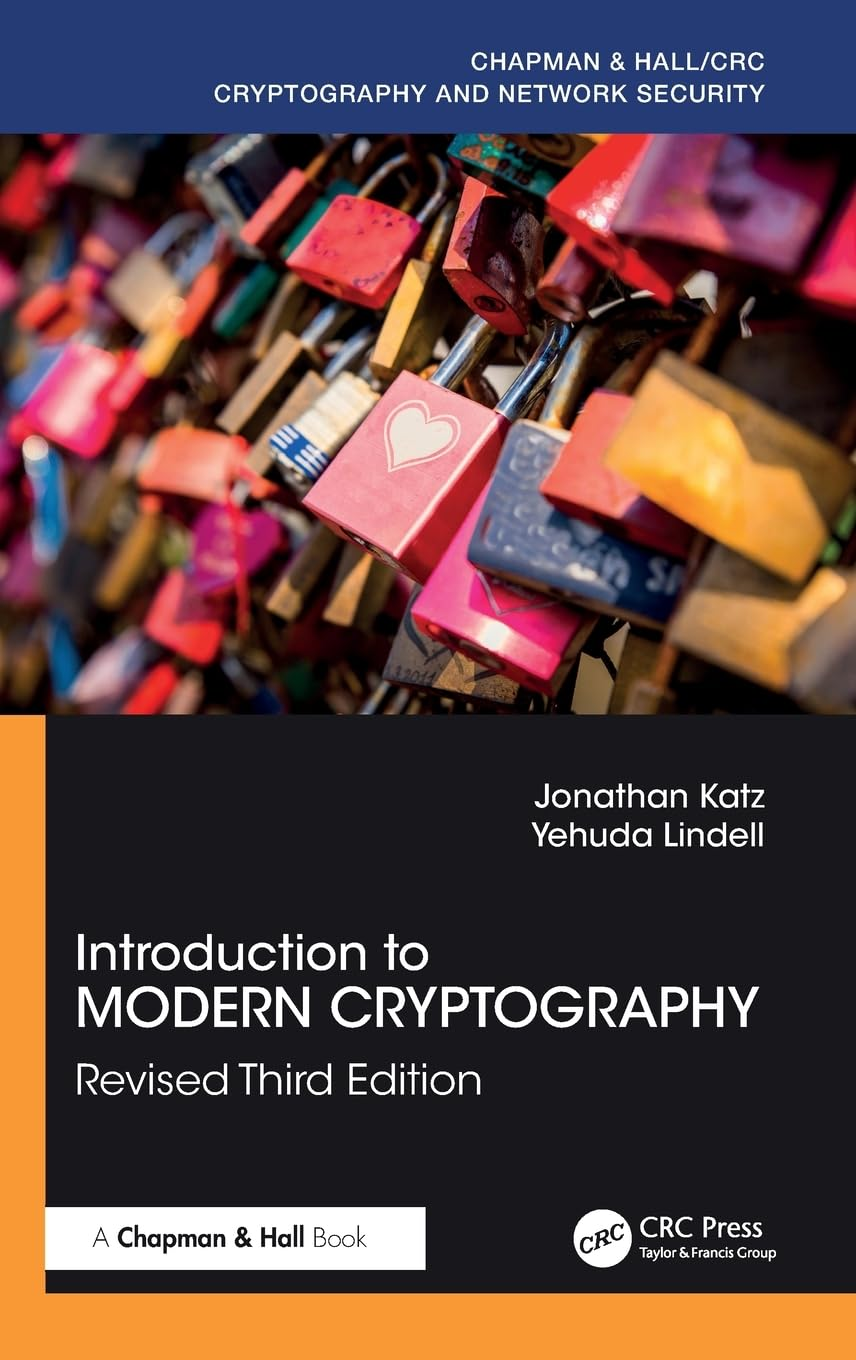
\includegraphics[scale=0.15]{images/katzlindell.png}}
  \end{center}
\item Slides adapted from Myrto Arapinis and beamer style curtely to Nadim Kobeissi \\ \url{https://appliedcryptography.page}
\end{itemize}
\end{frame}

\begin{frame}{What is cryptography?}
  
  \begin{block}{}
  \begin{quote}
    ``The practice of creating and understanding codes that keep information secret.''
  \end{quote}
  \hfill\small{Cambridge dictionary}
\end{block}
  \pause
  \bigskip
  \bigskip

  But nowadays cryptography encompasses many more things than just secret communications.
  \medskip

  \begin{block}{}
    \begin{quote}
      ``Cryptography is the scientific study of techniques for securing [against internal or external attacks] digital information, transactions, and distributed computations.''
    \end{quote}
    \hfill\small{Jonathan Katz and Yehuda Lindell} \\
    \hfill\small{in Introduction to Modern Cryptography}
  \end{block}
\end{frame}

\begin{frame}{Cryptography is everywhere!}

  Cryptographic methods are powerful tools at the core of many security mechanisms used:
  \begin{itemize}
  \item to securely and confidentially access a website such as an online banking website;
  \item to attest the identity of the organization operating a web server;
  \item when talking over a mobile phone;
  \item to enforce access control in a multi-user operating system;
  \item to prevent thieves extracting trade secrets from stolen laptops;
  \item to prevent software copying;
  \item \emph{etc}
  \end{itemize}
  \bigskip

  \begin{block}{}
    Cryptography (and security more broadly) is becoming a more and more central topic within computer science
  \end{block}
  
\end{frame}

\begin{frame}{Important remark}

  \bigskip
  
  \begin{alertblock}{Cryptography is not:}
    \begin{itemize}
    \item The solution to all security problems (see other sections of the course)\medskip
    \item Secure if not implemented and/or deployed correctly\medskip
    \item Something you will be able to invent at the end of this course
    \end{itemize}
  \end{alertblock}
  
\end{frame}

\begin{frame}{Learning objectives for the Cryptography section}

  \begin{itemize}
  \item Appreciate the variety of applications that use cryptography with different purposes
    \bigskip{}
    
  \item Introduce the basic concepts of cryptography
    \bigskip{}
    
    
  \item Understand the type of problems cryptography can address
    \bigskip{}
    
  \item Understand the types of problems that need to be addressed when using cryptography
    
  \end{itemize}

\end{frame}

\begin{frame}{Topics in the Cryptography section}
  We will discuss constructions for:
  \begin{itemize}
  \item Symmetric Encryption
  \item Asymmetric (public-key) Encryption
  \item Hash functions and Message Authentication Codes (MACs)
  \item Digital Signatures
  \item Public Key Infrastructure (PKI)
  \end{itemize}
  \bigskip
  \bigskip
  
  \begin{block}{We present only the rudiments of the topic:}
    \begin{itemize}
    \item What cryptography can achieve
    \item That cryptography can go wrong
    \item What is good practice when using cryptography
    \end{itemize}
  \end{block}
  
\end{frame}

\title{Cryptography: Symmetric encryption}
\covertopicname{Symmetric encryption}
\author{}
\date{}

\begin{frame}
  \titlepage
\end{frame}

\begin{frame}{Goal: confidentiality}\bigskip
  
  \begin{itemize}
  \item Secure communications
    \medskip
    \begin{center}
      \begin{tabular}{m{4.45cm}m{2cm}m{2cm}}
        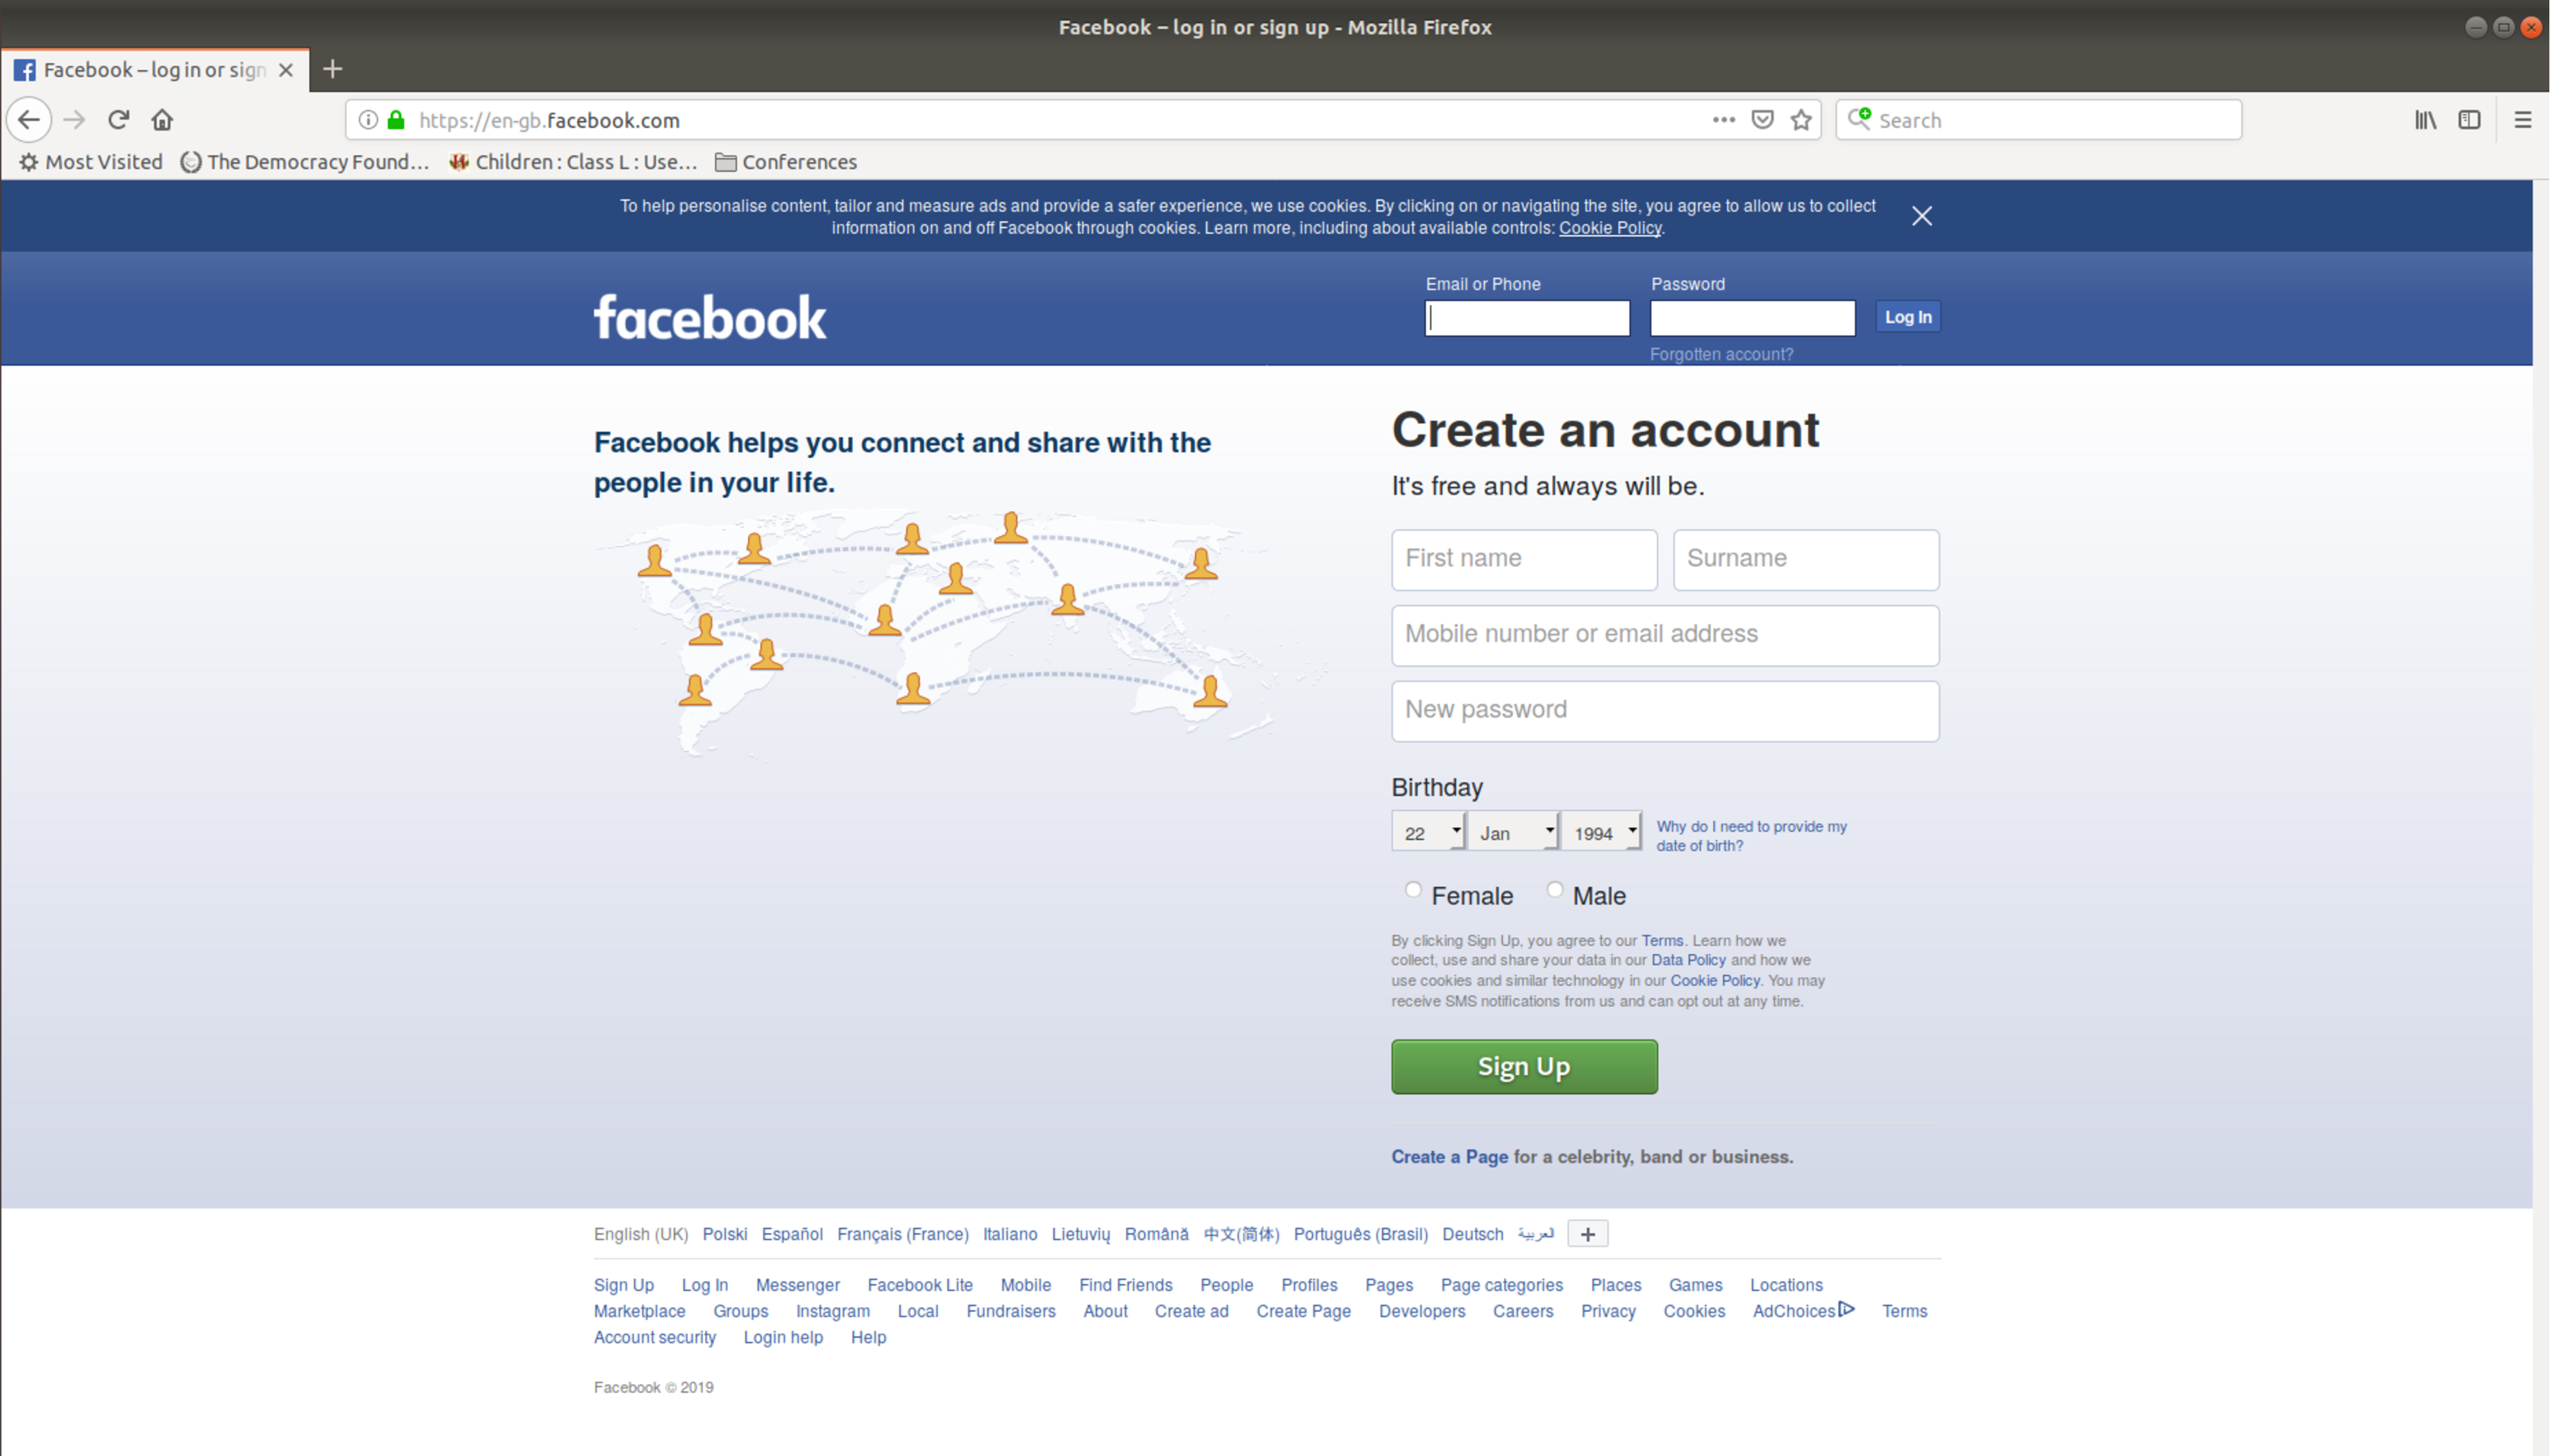
\includegraphics[scale=0.075]{Images/facebook.pdf} & 
\includegraphics[scale=0.25]{Images/encrypted-channel.pdf} & 
\includegraphics[scale=0.2]{Images/laptop.pdf}
      \end{tabular}
    \end{center}
    \bigskip

  \item File protection
    \medskip
    \begin{center}
      
\includegraphics[scale=0.09]{Images/file-protection.pdf}
    \end{center}
  \end{itemize}
\end{frame}

\begin{frame}{Symmetric encryption schemes}
  \vspace{-0.5cm}
  \begin{block}{}
    A symmetric cipher consists of two algorithms
    \begin{itemize}
    \item encryption algorithm $E:\ \mathcal{K} \times \mathcal{M} \rightarrow \mathcal{C}$
      
    \item decryption algorithm $D:\ \mathcal{K} \times \mathcal{C} \rightarrow \mathcal{M}$
    \end{itemize}
    st. $\forall k\in\mathcal{K}$, and $\forall m\in\mathcal{M}$, $D(k, E(k, m))\ =\ m$
  \end{block}
  
  \begin{center}
    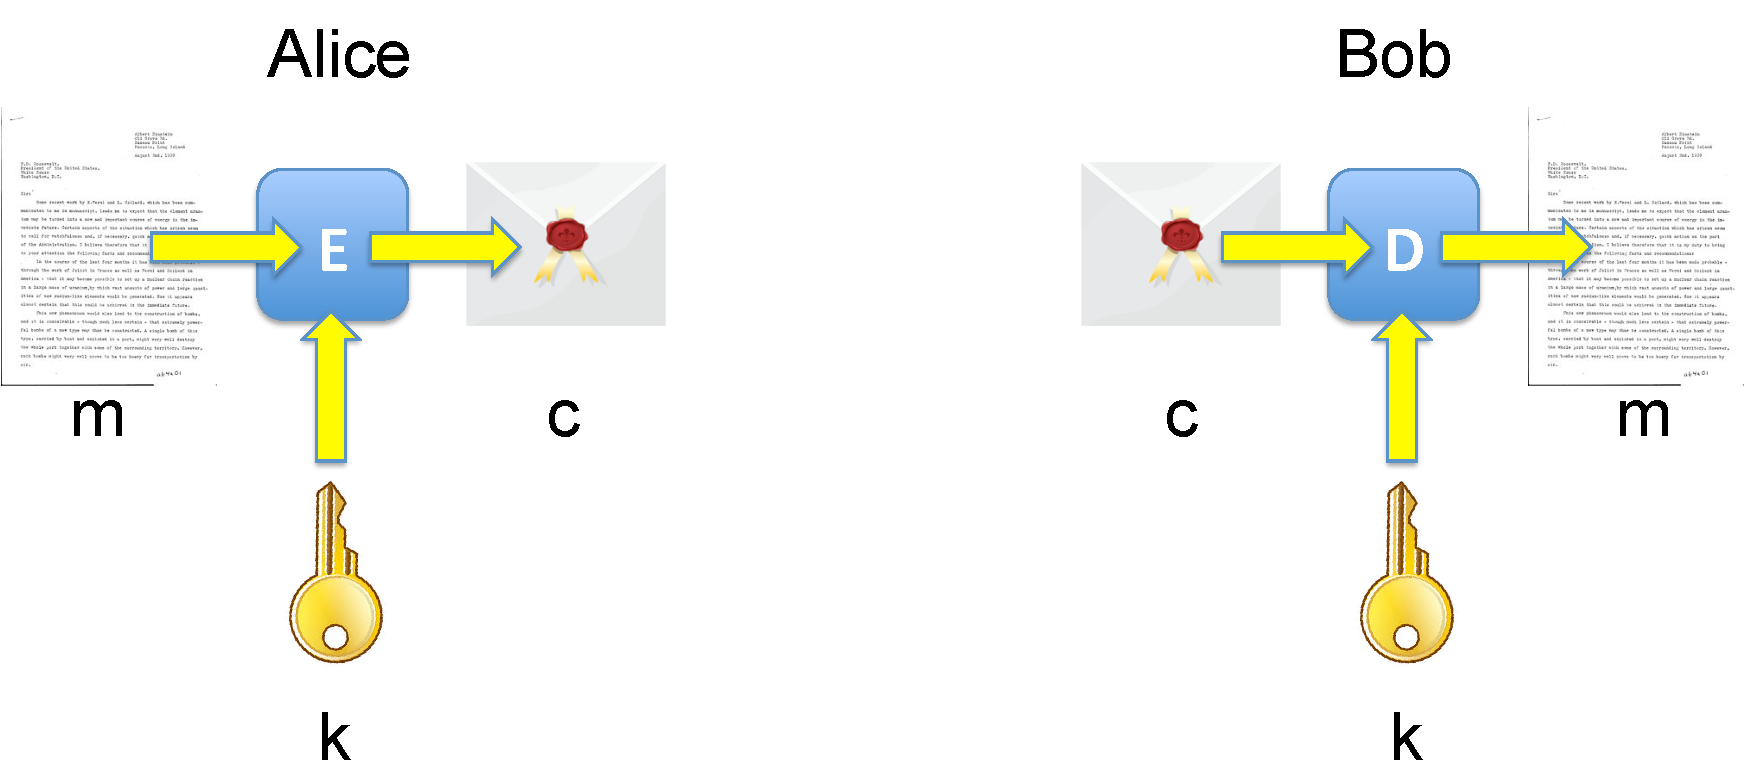
\includegraphics[scale=0.23]{Images/encryptA.pdf}
  \end{center}
  \begin{itemize}
  \item same key $k$ to encrypt and decrypt
  \item the key $k$ is secret: only known to Alice and Bob 
  \end{itemize}
  
\end{frame}

\begin{frame}{What is a good encryption scheme?}

  An encryption scheme is secure against a given adversary, if this adversary cannot
  
  \begin{itemize}
  \pause
  \item recover the secret key $k$
  \pause
  \item recover the plaintext $m$ underlying a ciphertext $c$
  \pause
  \item recover any bits of the plaintext $m$ underlying a ciphertext $c$
  \item \dots    
  \end{itemize}
\end{frame}

\begin{frame}{Kerckhoff's principle}

  The architecture and design of a security system/mechanism should be made public
  \bigskip
  
  \begin{alertblock}{No security through obscurity!}
    \begin{itemize}
    \item The encryption ($E$) and decryption ($D$) algorithms are public
    \item The security relies entirely on the secrecy of the key
    \end{itemize}
  \end{alertblock}
  \bigskip

  Open design allows for a system to be scrutinized by many users, white hat hackers, academics, \emph{etc.}

  \enrouge{$\rightsquigarrow$} early discovery and corrections of flaws/vulnerabilities  
\end{frame}

\begin{frame}{Adversary's capabilities}
  \vspace{-0.5cm}
  \begin{alertblock}{}
    \begin{itemize}
    \item[$\bullet$] A cryptographic scheme is secure under some assumptions, that is against a certain type of attacker
    \item[$\bullet$] A cryptographic scheme may be vulnerable to certain types of attacks but not others
    \end{itemize}
  \end{alertblock}
  \medskip
  \pause
  
  The attacker know the encryption/decryption algorithms but may have access to :
  \begin{itemize}
  \item \Inblue{Ciphertext only attack} - some ciphertexts $c_1$, \ldots, $c_n$
    \medskip

\pause    
  \item \Inblue{Known plaintext attack} some plaintext/ciphertext pairs $(m_1, c_1)$, \ldots, $(m_n, c_n)$ st. $c_i = E(k, m_i))$
    \medskip
  
  \pause  
  \item \Inblue{Chosen plaintext attack} - he has access to an encryption oracle - can maybe trick a user to encrypt messages $m_1$, \dots, $m_n$ of his choice
    \medskip

\pause
  \item \Inblue{Chosen ciphertext attack} - he has access to a decryption oracle - can maybe trick a user to decrypt ciphertexts $c_1$, \dots, $c_n$ of his choice
    \medskip

  \item unlimited, or polynomial, or realistic ($\le 2^{80}$) \Inblue{computational power}

  \end{itemize}

\end{frame}

\begin{frame}{Brute-force attack - attack on all schemes}
  \begin{itemize}
  \item Try all possible keys $k\in\mathcal{K}$ - requires some knowledge about the structure of plaintext
    \begin{center}
      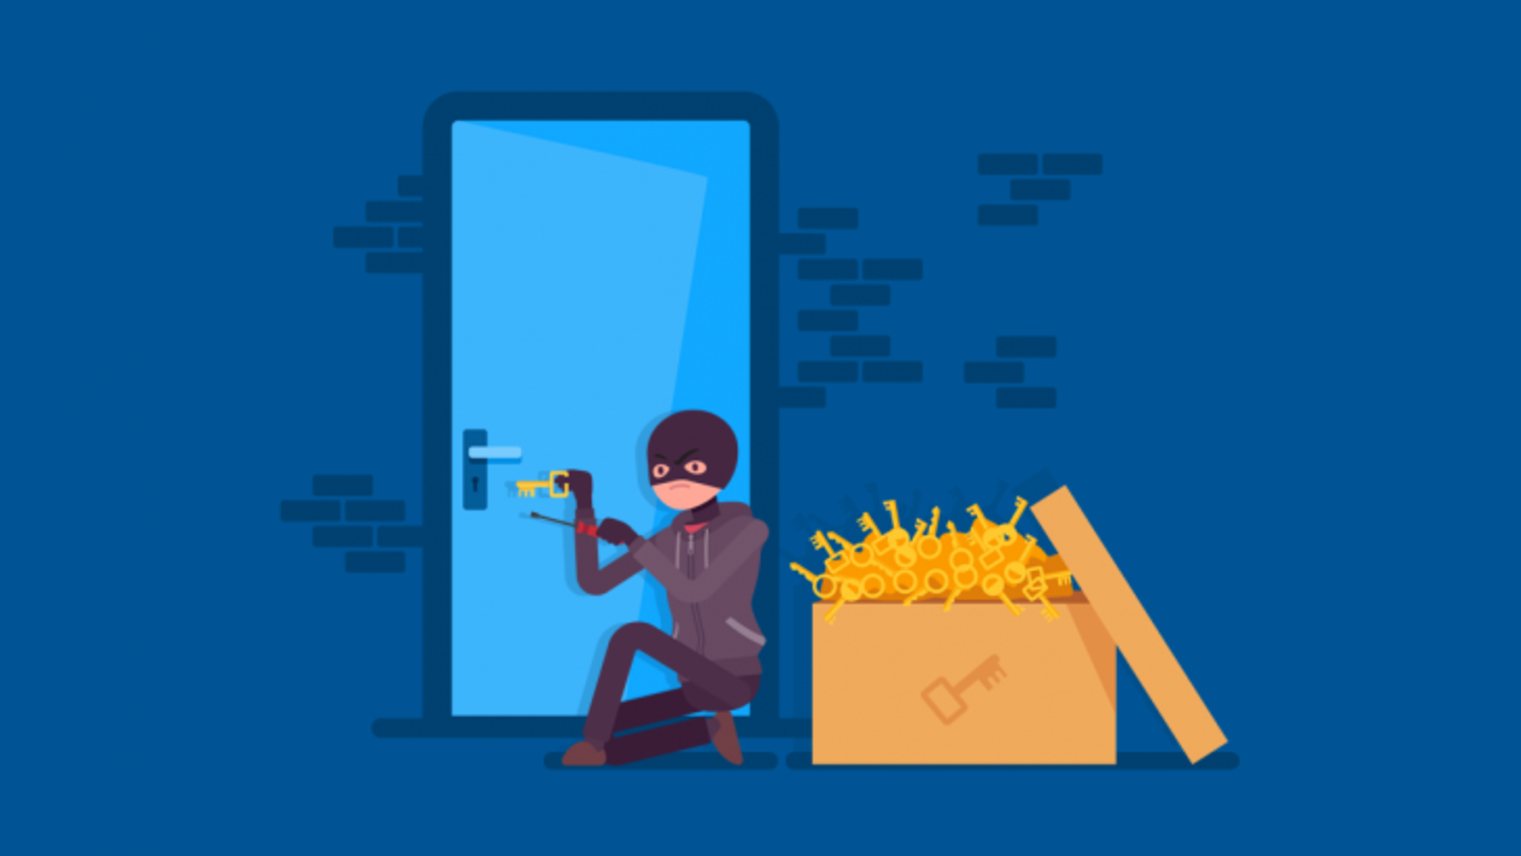
\includegraphics[scale=0.25]{Images/brute-force-attack.pdf}
    \end{center}
    \bigskip
    
  \item Making exhaustive search unfeasible:
    \begin{itemize}
    \item $\mathcal K$ should be sufficiently large, \emph{i.e.} keys
      should be sufficiently long
    \item Keys should be sampled uniformly at random from $\mathcal K$
  \end{itemize}

  \end{itemize}
\end{frame}

\begin{frame}{A simple scheme: the substitution cipher}

  \begin{itemize}
  \item shared secret: a permutation $\pi$ of the set of characters

    \enrouge{
      \small{$\pi=
        \begin{array}[t]{l}
          a\mapsto q\ b\mapsto w\ c\mapsto e\ d\mapsto r\ e\mapsto t\ f\mapsto y\ g\mapsto u\ h\mapsto i\ 
          i\mapsto o \\ 
          j\mapsto m\ k\mapsto a\ l\mapsto s\ m\mapsto d\ n\mapsto f\ o\mapsto g\ p\mapsto h\ q\mapsto j\ r\mapsto k \\ 
          s\mapsto l\ t\mapsto z\ u\mapsto x\ v\mapsto c\ w\mapsto v\ x\mapsto b\ y\mapsto n\ z\mapsto p\
        \end{array}
        $}}
    \normalsize
    \vspace{0.5cm}

  \item Encryption: apply $\pi$ to each character of the plaintext
    \[
    E(\enrouge{\pi}, \enbleu{p_1\dots p_n})\ = \ \enrouge{\pi}(\enbleu{p_1})\dots\enrouge{\pi}(\enbleu{p_n})
    \]
    \vspace{0.15cm}

  \item Decryption: apply $\pi^{-1}$ to each character of the plaintext
    \[
    D(\enrouge{\pi}, \envert{c_1\dots c_n})\ = \ \enrouge{\pi^{-1}}(\envert{c_1})\dots\enrouge{\pi^{-1}}(\envert{c_n})
    \]
  \end{itemize}
\end{frame}

\begin{frame}{Substitution cipher: example}
  \vspace{-0.7cm}
    \enrouge{
    \scriptsize{$\pi=
      \begin{array}[t]{l}
        a\mapsto q\ b\mapsto w\ c\mapsto e\ d\mapsto r\ e\mapsto t\ f\mapsto y\ g\mapsto u\ h\mapsto i\ 
        i\mapsto o\ j\mapsto m\ k\mapsto a\ l\mapsto s \\ 
        m\mapsto d\ n\mapsto f\ o\mapsto g\ p\mapsto h\ q\mapsto j\ r\mapsto k\ s\mapsto l\ t\mapsto z\ 
        u\mapsto x\ v\mapsto c\ w\mapsto v\ x\mapsto b\  
        y\mapsto n\ z\mapsto p\
      \end{array}
      $}}
  \vspace{0.10cm}
  
  \enbleu{
    \scriptsize{m =
      \begin{tabular}[t]{l}
        THIS COURSE AIMS TO INTRODUCE YOU TO THE PRINCIPLES AND TECHNIQUES OF\\ 
        SECURING COMPUTERS AND COMPUTER NETWORKS WITH FOCUS ON INTERNET \\
        SECURITY. THE COURSE IS EFFECTIVELY SPLIT INTO TWO PARTS. FIRST INTRODUCING \\ 
       THE THEORY OF CRYPTOGRAPHY INCLUDING HOW MANY CLASSICAL AND POPULAR \\
        ALGORITHMS WORK E.G. DES, RSA, DIGITAL SIGNATURES, AND SECOND PROVIDING\\
         DETAILS OF REAL INTERNET SECURITY PROTOCOLS, ALGORITHMS, AND THREATS,\\
         E.G. IPSEC, VIRUSES, FIREWALLS. HENCE, YOU WILL LEARN BOTH THEORETICAL\\
        ASPECTS OF COMPUTER AND NETWORK SECURITY AS WELL AS HOW THAT THEORY IS \\
        APPLIED IN THE INTERNET. THIS KNOWLEDGE WILL HELP YOU IN DESIGNING AND \\ DEVELOPING SECURE APPLICATIONS AND NETWORK PROTOCOLS AS WELL AS 
        BUILDING \\ 
        SECURE NETWORKS.
      \end{tabular}
    }}
  \vspace{0.10cm}
  
  \envert{
    \scriptsize{c =
      \begin{tabular}[t]{l}
        ZIOL EGXKLT QODL ZG OFZKGRXET NGX ZG ZIT HKOFEOHSTL QFR ZTEIFOJXTL GY \\
        LTEXKOFU EGDHXZTKL QFR EGDHXZTK FTZVGKAL VOZI YGEXL GF OFZTKFTZ \\
        LTEXKOZN. ZIT EGXKLT OL TYYTEZOCTSN LHSOZ OFZG ZVG HQKZL. YOKLZ OFZKGRXEOFU \\
        ZIT ZITGKN GY EKNHZGUKQHIN OFESXROFU IGV DQFN ESQLLOEQS QFR HGHXSQK \\
        QSUGKOZIDL VGKA T.U. RTL, KLQ, ROUOZQS LOUFQZXKTL, QFR LTEGFR HKGCOROFU\\
        RTZQOSL GY KTQS OFZTKFTZ LTEXKOZN HKGZGEGSL, QSUGKOZIDL, QFR ZIKTQZL,\\
        T.U. OHLTE, COKXLTL, YOKTVQSSL. ITFET, NGX VOSS STQKF WGZI ZITGKTZOEQS\\
        QLHTEZL GY EGDHXZTK QFR FTZVGKA LTEXKOZN QL VTSS QL IGV ZIQZ ZITGKN OL\\
        QHHSOTR OF ZIT OFZTKFTZ. ZIOL AFGVSTRUT VOSS ITSH NGX OF RTLOUFOFU QFR\\
       RTCTSGHOFU LTEXKT QHHSOEQZOGFL QFR FTZVGKA HKGZGEGSL QL VTSS QL WXOSROFU\\
       LTEXKT FTZVGKAL.
      \end{tabular}
    }}
\end{frame}

\title{Quiz}
\author{}
\date{}
\begin{frame}{}
%  \coverpartname{Cryptography}
\covertopicname{Quiz}
\titlepage  
\end{frame}

\begin{frame}
  \frametitle{Breaking the substitution cipher}
  \pause
\vspace{-0.5cm}
  \begin{itemize}
  \item Key space size: $|\mathcal{K}| = 26!\ (\approx 2^{88})$
    \hfill\enrouge{$\Rightarrow$ brute force infeasible!}
    \vspace{0.25cm}
    \pause
    
  \item \enrouge{Frequency analysis:} exploit regularities of the language
    \begin{itemize}
    \item Use frequency of letters in English text
      \begin{center}
        \begin{tabular}[t]{c}
          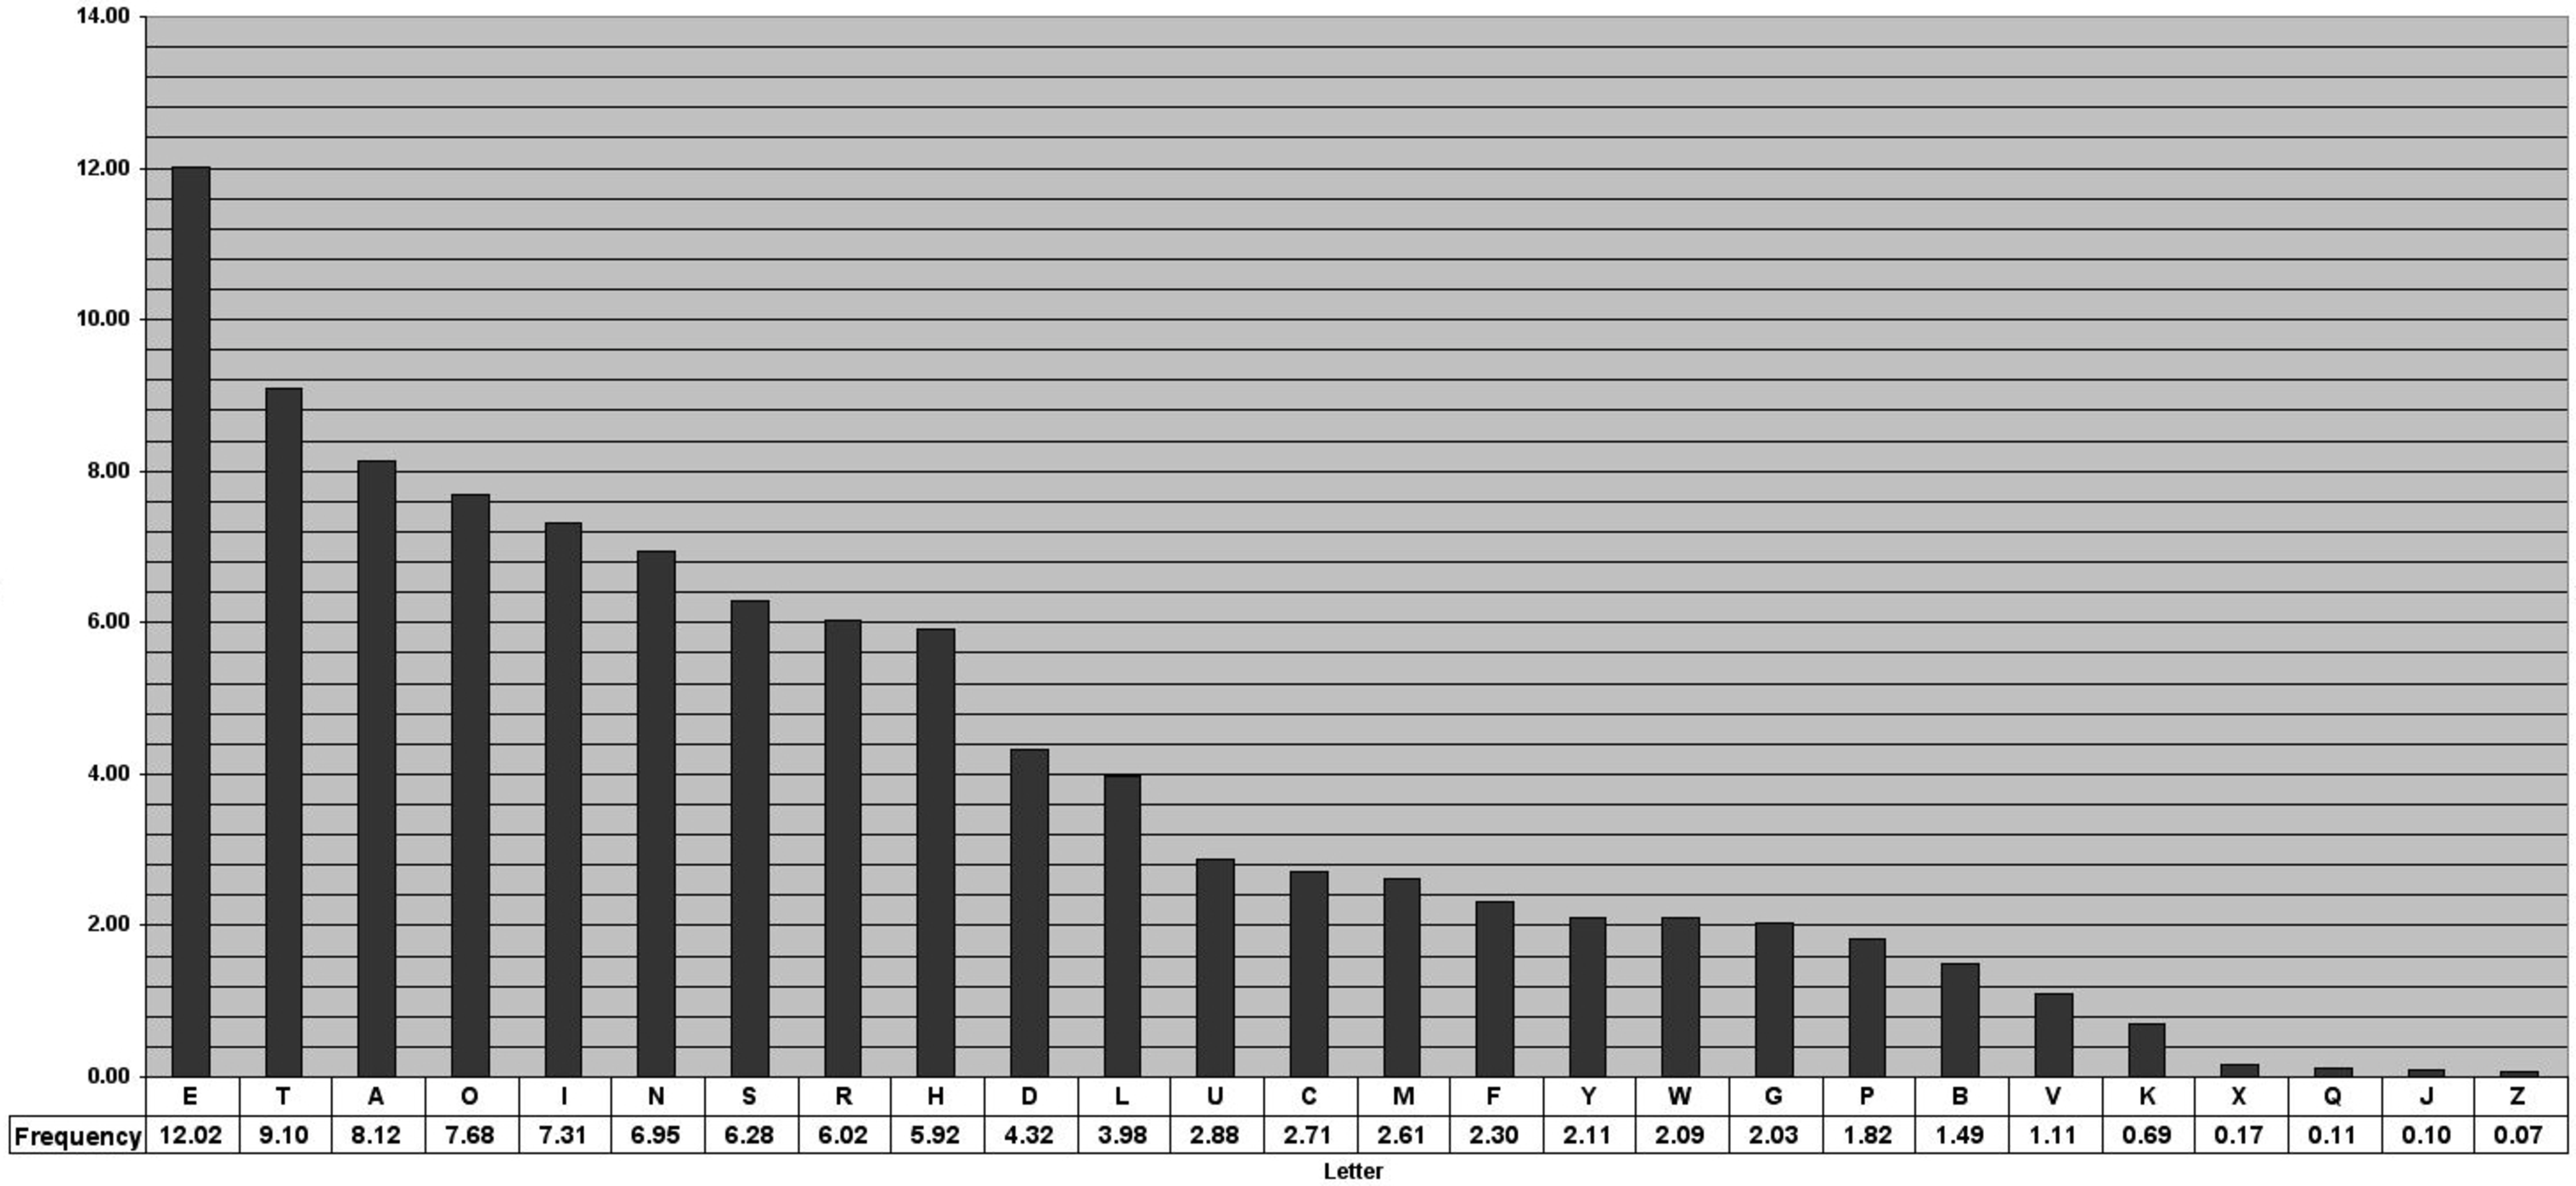
\includegraphics[scale=0.09]{Images/frequency.pdf} 
          
        \end{tabular}
      \end{center}
        
    \item Use frequency of digrams in English text
      \begin{center}
        \begin{tabular}[t]{c}
          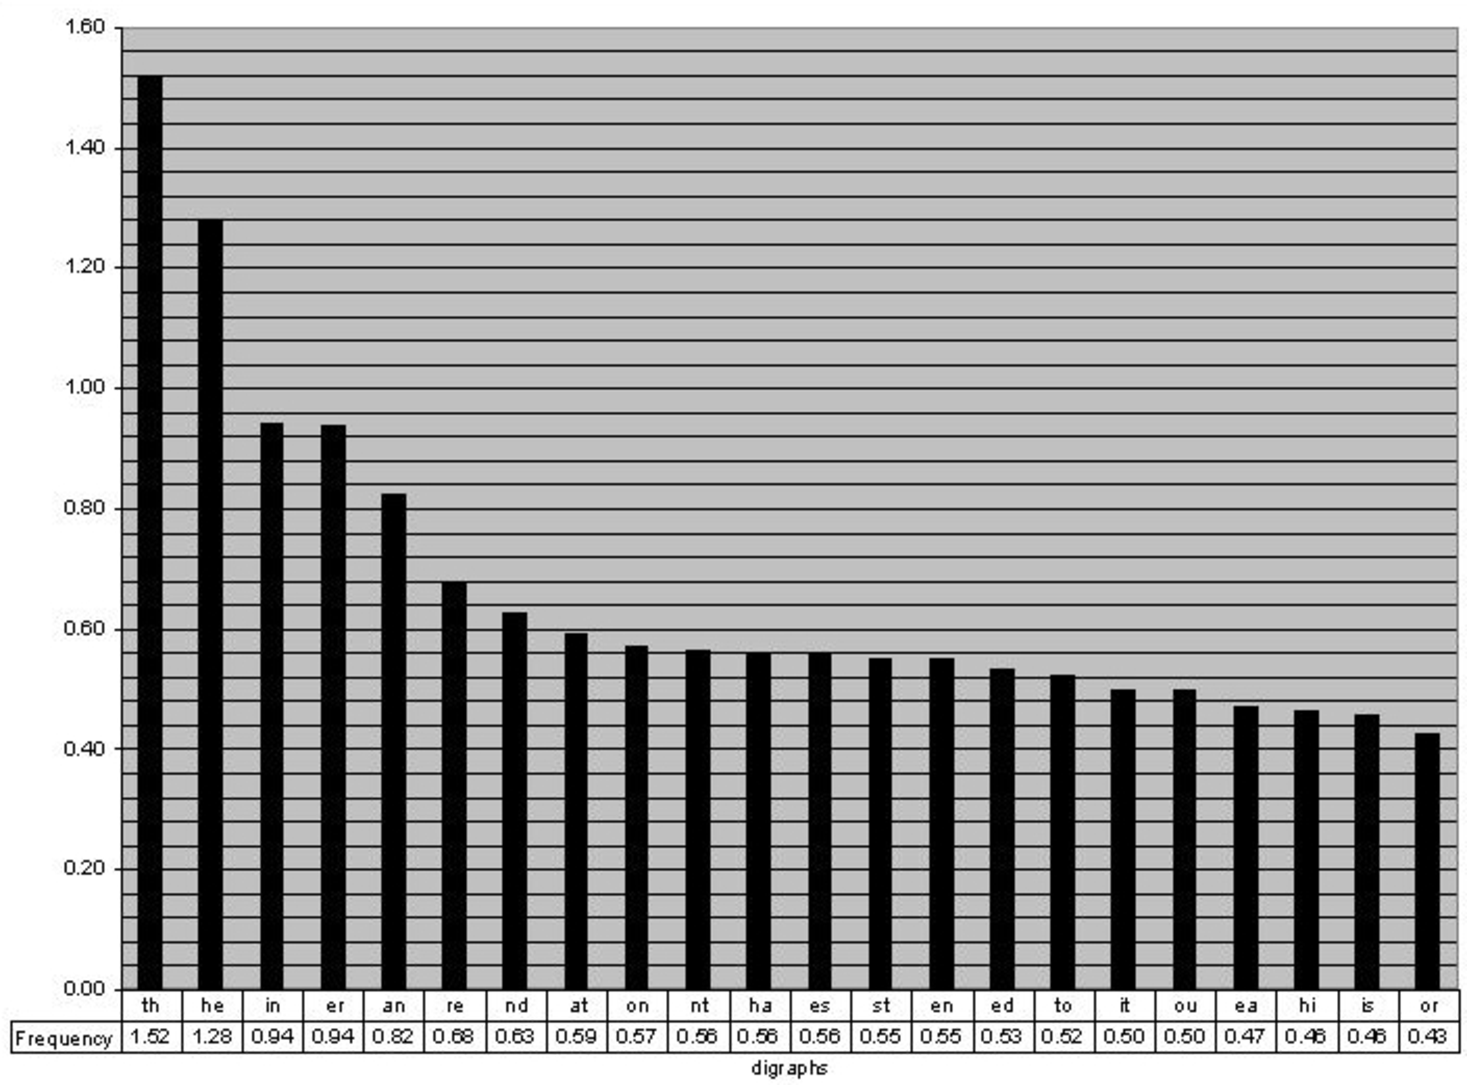
\includegraphics[scale=0.10]{Images/digraphs.pdf}
          
        \end{tabular}
      \end{center}
    \item Use frequency of trigrams in English text
      \begin{center}
        \envert{the $>$ and $>$ ing}
      \end{center}
      
    \item Use expected words
    \end{itemize}
  \end{itemize}

\end{frame}

\begin{frame}{Breaking the substitution cipher: example}

  \enrouge{
    \tiny{$\pi=
      $}}
  \vspace{0.25cm}

  
  \color{vert}
  \tiny{c =
    \begin{tabular}[t]{l}
      ZIOL EGXKLT QODL ZG OFZKGRXET NGX ZG ZIT HKOFEOHSTL QFR ZTEIFOJXTL GY \\
      LTEXKOFU EGDHXZTKL QFR EGDHXZTK FTZVGKAL VOZI YGEXL GF OFZTKFTZ \\
      LTEXKOZN. ZIT EGXKLT OL TYYTEZOCTSN LHSOZ OFZG ZVG HQKZL. YOKLZ \\
      OFZKGRXEOFU ZIT ZITGKN GY EKNHZGUKQHIN OFESXROFU IGV DQFN ESQLLOEQS \\
      QFR HGHXSQK QSUGKOZIDL VGKA T.U. RTL, KLQ, ROUOZQS LOUFQZXKTL, QFR \\
      LTEGFR HKGCOROFU RTZQOSL GY KTQS OFZTKFTZ LTEXKOZN HKGZGEGSL, \\
      QSUGKOZIDL, QFR ZIKTQZL, T.U. OHLTE, COKXLTL, YOKTVQSSL. ITFET, NGX \\
      VOSS STQKF WGZI ZITGKTZOEQS QLHTEZL GY EGDHXZTK QFR FTZVGKA \\
      LTEXKOZN QL VTSS QL IGV ZIQZ ZITGKN OL QHHSOTR OF ZIT OFZTKFTZ. ZIOL \\
      AFGVSTRUT VOSS ITSH NGX OF RTLOUFOFU QFR RTCTSGHOFU LTEXKT \\
      QHHSOEQZOGFL QFR FTZVGKA HKGZGEGSL QL VTSS QL WXOSROFU LTEXKT \\
      FTZVGKAL.
    \end{tabular}
  }
  \vspace{0.5cm}

  \normalsize
  
\end{frame}

\begin{frame}
  \frametitle{Breaking the substitution cipher: example}

  \enrouge{
    \tiny{$\pi=
      $}}
  \vspace{0.25cm}

  
  \color{vert}
  \tiny{c =
    \begin{tabular}[t]{l}
      ZIOL EGXKLT QODL ZG OFZKGRXET NGX ZG ZIT HKOFEOHSTL QFR ZTEIFOJXTL GY \\
      LTEXKOFU EGDHXZTKL QFR EGDHXZTK FTZVGKAL VOZI YGEXL GF OFZTKFTZ \\
      LTEXKOZN. ZIT EGXKLT OL TYYTEZOCTSN LHSOZ OFZG ZVG HQKZL. YOKLZ \\
      OFZKGRXEOFU ZIT ZITGKN GY EKNHZGUKQHIN OFESXROFU IGV DQFN ESQLLOEQS \\
      QFR HGHXSQK QSUGKOZIDL VGKA T.U. RTL, KLQ, ROUOZQS LOUFQZXKTL, QFR \\
      LTEGFR HKGCOROFU RTZQOSL GY KTQS OFZTKFTZ LTEXKOZN HKGZGEGSL, \\
      QSUGKOZIDL, QFR ZIKTQZL, T.U. OHLTE, COKXLTL, YOKTVQSSL. ITFET, NGX \\
      VOSS STQKF WGZI ZITGKTZOEQS QLHTEZL GY EGDHXZTK QFR FTZVGKA \\
      LTEXKOZN QL VTSS QL IGV ZIQZ ZITGKN OL QHHSOTR OF ZIT OFZTKFTZ. ZIOL \\
      AFGVSTRUT VOSS ITSH NGX OF RTLOUFOFU QFR RTCTSGHOFU LTEXKT \\
      QHHSOEQZOGFL QFR FTZVGKA HKGZGEGSL QL VTSS QL WXOSROFU LTEXKT \\
      FTZVGKAL.
    \end{tabular}
  }
  \vspace{0.5cm}

  \normalsize
  \color{black}{Most common letters in c: t $>$ z $>$ o $>$ l}
\end{frame}


\begin{frame}
  \frametitle{Breaking the substitution cipher: example}

    \enrouge{
    \tiny{$\pi=
      \begin{array}[t]{l}
      t\mapsto z\ e\mapsto t\
      \end{array}
      $}}
  \vspace{0.25cm}
  
  \color{vert}
  \tiny{c =
    \begin{tabular}[t]{l}
      \enbleu{T}IOL EGXKL\enbleu{E} QODL \enbleu{T}G OF\enbleu{T}KGRXE\enbleu{E} NGX \enbleu{T}G \enbleu{T}I\enbleu{E} HKOFEOHS\enbleu{E}L QFR \enbleu{T}\enbleu{E}EIFOJX\enbleu{E}L GY \\
      L\enbleu{E}EXKOFU EGDHX\enbleu{T}\enbleu{E}KL QFR EGDHX\enbleu{T}\enbleu{E}K F\enbleu{E}\enbleu{T}VGKAL VO\enbleu{T}I YGEXL GF OF\enbleu{T}\enbleu{E}KF\enbleu{E}\enbleu{T} \\
      L\enbleu{E}EXKO\enbleu{T}N. \enbleu{T}I\enbleu{E} EGXKL\enbleu{E} OL \enbleu{E}YY\enbleu{E}E\enbleu{T}OC\enbleu{E}SN LHSO\enbleu{T} OF\enbleu{T}G \enbleu{T}VG HQK\enbleu{T}L. YOKL\enbleu{T} \\
      OF\enbleu{T}KGRXEOFU \enbleu{T}I\enbleu{E} \enbleu{T}I\enbleu{E}GKN GY EKNH\enbleu{T}GUKQHIN OFESXROFU IGV DQFN ESQLLOEQS \\
      QFR HGHXSQK QSUGKO\enbleu{T}IDL VGKA \enbleu{E}.U. R\enbleu{E}L, KLQ, ROUO\enbleu{T}QS LOUFQ\enbleu{T}XK\enbleu{E}L, QFR \\
      L\enbleu{E}EGFR HKGCOROFU R\enbleu{E}\enbleu{T}QOSL GY K\enbleu{E}QS OF\enbleu{T}\enbleu{E}KF\enbleu{E}\enbleu{T} L\enbleu{E}EXKO\enbleu{T}N HKG\enbleu{T}GEGSL, \\
      QSUGKO\enbleu{T}IDL, QFR \enbleu{T}IK\enbleu{E}Q\enbleu{T}L, \enbleu{E}.U. OHL\enbleu{E}E, COKXL\enbleu{E}L, YOK\enbleu{E}VQSSL. I\enbleu{E}FE\enbleu{E}, NGX \\
      VOSS S\enbleu{E}QKF WG\enbleu{T}I \enbleu{T}I\enbleu{E}GK\enbleu{E}\enbleu{T}OEQS QLH\enbleu{E}E\enbleu{T}L GY EGDHX\enbleu{T}\enbleu{E}K QFR F\enbleu{E}\enbleu{T}VGKA \\
      L\enbleu{E}EXKO\enbleu{T}N QL V\enbleu{E}SS QL IGV \enbleu{T}IQ\enbleu{T} \enbleu{T}I\enbleu{E}GKN OL QHHSO\enbleu{E}R OF \enbleu{T}I\enbleu{E} OF\enbleu{T}\enbleu{E}KF\enbleu{E}\enbleu{T}. \enbleu{T}IOL \\
      AFGVS\enbleu{E}RU\enbleu{E} VOSS I\enbleu{E}SH NGX OF R\enbleu{E}LOUFOFU QFR R\enbleu{E}C\enbleu{E}SGHOFU L\enbleu{E}EXK\enbleu{E} \\
      QHHSOEQ\enbleu{T}OGFL QFR F\enbleu{E}\enbleu{T}VGKA HKG\enbleu{T}GEGSL QL V\enbleu{E}SS QL WXOSROFU L\enbleu{E}EXK\enbleu{E} \\
      F\enbleu{E}\enbleu{T}VGKAL.
    \end{tabular}
  }
  \vspace{0.5cm}

  \normalsize
  \color{black}Most common letters in c: t $>$ z $>$ \dots
  
  \color{black}
\end{frame}

\begin{frame}
  \frametitle{Breaking the substitution cipher: example}

    \enrouge{
    \tiny{$\pi=
      \begin{array}[t]{l}
      t\mapsto z\ e\mapsto t\
      \end{array}
      $}}
  \vspace{0.25cm}
  
  \color{vert}
  \tiny{c =
    \begin{tabular}[t]{l}
      \enbleu{T}IOL EGXKL\enbleu{E} QODL \enbleu{T}G OF\enbleu{T}KGRXE\enbleu{E} NGX \enbleu{T}G \enbleu{T}I\enbleu{E} HKOFEOHS\enbleu{E}L QFR \enbleu{T}\enbleu{E}EIFOJX\enbleu{E}L GY \\
      L\enbleu{E}EXKOFU EGDHX\enbleu{T}\enbleu{E}KL QFR EGDHX\enbleu{T}\enbleu{E}K F\enbleu{E}\enbleu{T}VGKAL VO\enbleu{T}I YGEXL GF OF\enbleu{T}\enbleu{E}KF\enbleu{E}\enbleu{T} \\
      L\enbleu{E}EXKO\enbleu{T}N. \enbleu{T}I\enbleu{E} EGXKL\enbleu{E} OL \enbleu{E}YY\enbleu{E}E\enbleu{T}OC\enbleu{E}SN LHSO\enbleu{T} OF\enbleu{T}G \enbleu{T}VG HQK\enbleu{T}L. YOKL\enbleu{T} \\
      OF\enbleu{T}KGRXEOFU \enbleu{T}I\enbleu{E} \enbleu{T}I\enbleu{E}GKN GY EKNH\enbleu{T}GUKQHIN OFESXROFU IGV DQFN ESQLLOEQS \\
      QFR HGHXSQK QSUGKO\enbleu{T}IDL VGKA \enbleu{E}.U. R\enbleu{E}L, KLQ, ROUO\enbleu{T}QS LOUFQ\enbleu{T}XK\enbleu{E}L, QFR \\
      L\enbleu{E}EGFR HKGCOROFU R\enbleu{E}\enbleu{T}QOSL GY K\enbleu{E}QS OF\enbleu{T}\enbleu{E}KF\enbleu{E}\enbleu{T} L\enbleu{E}EXKO\enbleu{T}N HKG\enbleu{T}GEGSL, \\
      QSUGKO\enbleu{T}IDL, QFR \enbleu{T}IK\enbleu{E}Q\enbleu{T}L, \enbleu{E}.U. OHL\enbleu{E}E, COKXL\enbleu{E}L, YOK\enbleu{E}VQSSL. I\enbleu{E}FE\enbleu{E}, NGX \\
      VOSS S\enbleu{E}QKF WG\enbleu{T}I \enbleu{T}I\enbleu{E}GK\enbleu{E}\enbleu{T}OEQS QLH\enbleu{E}E\enbleu{T}L GY EGDHX\enbleu{T}\enbleu{E}K QFR F\enbleu{E}\enbleu{T}VGKA \\
      L\enbleu{E}EXKO\enbleu{T}N QL V\enbleu{E}SS QL IGV \enbleu{T}IQ\enbleu{T} \enbleu{T}I\enbleu{E}GKN OL QHHSO\enbleu{E}R OF \enbleu{T}I\enbleu{E} OF\enbleu{T}\enbleu{E}KF\enbleu{E}\enbleu{T}. \enbleu{T}IOL \\
      AFGVS\enbleu{E}RU\enbleu{E} VOSS I\enbleu{E}SH NGX OF R\enbleu{E}LOUFOFU QFR R\enbleu{E}C\enbleu{E}SGHOFU L\enbleu{E}EXK\enbleu{E} \\
      QHHSOEQ\enbleu{T}OGFL QFR F\enbleu{E}\enbleu{T}VGKA HKG\enbleu{T}GEGSL QL V\enbleu{E}SS QL WXOSROFU L\enbleu{E}EXK\enbleu{E} \\
      F\enbleu{E}\enbleu{T}VGKAL.
    \end{tabular}
  }
  \vspace{0.5cm}

  \normalsize
  \color{black}Most common digrams in c: of $>$ zi $>$ \dots
  
  \pause

  t$\mapsto$z suggests h$\mapsto$i

  \color{black}
\end{frame}


\begin{frame}
  \frametitle{Breaking the substitution cipher: example}

  
    \enrouge{
    \tiny{$\pi=
      \begin{array}[t]{l}
      t\mapsto z\ e\mapsto t\ h\mapsto i\ 
      \end{array}
      $}}
  \vspace{0.25cm}

  \color{vert}
  \tiny{c =
    \begin{tabular}[t]{l}
      \enbleu{T}\enbleu{H}OL EGXKL\enbleu{E} QODL \enbleu{T}G OF\enbleu{T}KGRXE\enbleu{E} NGX \enbleu{T}G \enbleu{T}\enbleu{H}\enbleu{E} HKOFEOHS\enbleu{E}L QFR \enbleu{T}\enbleu{E}E\enbleu{H}FOJX\enbleu{E}L GY \\
      L\enbleu{E}EXKOFU EGDHX\enbleu{T}\enbleu{E}KL QFR EGDHX\enbleu{T}\enbleu{E}K F\enbleu{E}\enbleu{T}VGKAL VO\enbleu{T}\enbleu{H} YGEXL GF OF\enbleu{T}\enbleu{E}KF\enbleu{E}\enbleu{T} \\
      L\enbleu{E}EXKO\enbleu{T}N. \enbleu{T}\enbleu{H}\enbleu{E} EGXKL\enbleu{E} OL \enbleu{E}YY\enbleu{E}E\enbleu{T}OC\enbleu{E}SN LHSO\enbleu{T} OF\enbleu{T}G \enbleu{T}VG HQK\enbleu{T}L. YOKL\enbleu{T} \\
      OF\enbleu{T}KGRXEOFU \enbleu{T}\enbleu{H}\enbleu{E} \enbleu{T}\enbleu{H}\enbleu{E}GKN GY EKNH\enbleu{T}GUKQH\enbleu{H}N OFESXROFU \enbleu{H}GV DQFN ESQLLOEQS \\
      QFR HGHXSQK QSUGKO\enbleu{T}\enbleu{H}DL VGKA \enbleu{E}.U. R\enbleu{E}L, KLQ, ROUO\enbleu{T}QS LOUFQ\enbleu{T}XK\enbleu{E}L, QFR \\
      L\enbleu{E}EGFR HKGCOROFU R\enbleu{E}\enbleu{T}QOSL GY K\enbleu{E}QS OF\enbleu{T}\enbleu{E}KF\enbleu{E}\enbleu{T} L\enbleu{E}EXKO\enbleu{T}N HKG\enbleu{T}GEGSL, \\
      QSUGKO\enbleu{T}\enbleu{H}DL, QFR \enbleu{T}\enbleu{H}K\enbleu{E}Q\enbleu{T}L, \enbleu{E}.U. OHL\enbleu{E}E, COKXL\enbleu{E}L, YOK\enbleu{E}VQSSL. \enbleu{H}\enbleu{E}FE\enbleu{E}, NGX \\
      VOSS S\enbleu{E}QKF WG\enbleu{T}\enbleu{H} \enbleu{T}\enbleu{H}\enbleu{E}GK\enbleu{E}\enbleu{T}OEQS QLH\enbleu{E}E\enbleu{T}L GY EGDHX\enbleu{T}\enbleu{E}K QFR F\enbleu{E}\enbleu{T}VGKA \\
      L\enbleu{E}EXKO\enbleu{T}N QL V\enbleu{E}SS QL \enbleu{H}GV \enbleu{T}\enbleu{H}Q\enbleu{T} \enbleu{T}\enbleu{H}\enbleu{E}GKN OL QHHSO\enbleu{E}R OF \enbleu{T}\enbleu{H}\enbleu{E} OF\enbleu{T}\enbleu{E}KF\enbleu{E}\enbleu{T}. \enbleu{T}\enbleu{H}OL \\
      AFGVS\enbleu{E}RU\enbleu{E} VOSS \enbleu{H}\enbleu{E}SH NGX OF R\enbleu{E}LOUFOFU QFR R\enbleu{E}C\enbleu{E}SGHOFU L\enbleu{E}EXK\enbleu{E} \\
      QHHSOEQ\enbleu{T}OGFL QFR F\enbleu{E}\enbleu{T}VGKA HKG\enbleu{T}GEGSL QL V\enbleu{E}SS QL WXOSROFU L\enbleu{E}EXK\enbleu{E} \\
      F\enbleu{E}\enbleu{T}VGKAL.
    \end{tabular}
  }
  \vspace{0.5cm}

  \color{black}\normalsize{Most common digrams in c: of $>$ zi $>$ \dots}
  \pause

  we guess in$\mapsto$of
  
  \color{black}
\end{frame}

\begin{frame}
  \frametitle{Breaking the substitution cipher: example}
  
    \enrouge{
    \tiny{$\pi=
      \begin{array}[t]{l}
      t\mapsto z\ e\mapsto t\ h\mapsto i\ i\mapsto o\ n\mapsto f
      \end{array}
      $}}
  \vspace{0.25cm}

  \color{vert}
  \tiny{c =
    \begin{tabular}[t]{l}
      \enbleu{T}\enbleu{H}\enbleu{I}L EGXKL\enbleu{E} Q\enbleu{I}DL \enbleu{T}G \enbleu{I}\enbleu{N}\enbleu{T}KGRXE\enbleu{E} NGX \enbleu{T}G \enbleu{T}\enbleu{H}\enbleu{E} HK\enbleu{I}\enbleu{N}E\enbleu{I}HS\enbleu{E}L Q\enbleu{N}R \enbleu{T}\enbleu{E}E\enbleu{H}\enbleu{N}\enbleu{I}JX\enbleu{E}L GY \\
      L\enbleu{E}EXK\enbleu{I}\enbleu{N}U EGDHX\enbleu{T}\enbleu{E}KL Q\enbleu{N}R EGDHX\enbleu{T}\enbleu{E}K \enbleu{N}\enbleu{E}\enbleu{T}VGKAL V\enbleu{I}\enbleu{T}\enbleu{H} YGEXL G\enbleu{N} \enbleu{I}\enbleu{N}\enbleu{T}\enbleu{E}K\enbleu{N}\enbleu{E}\enbleu{T} \\
      L\enbleu{E}EXK\enbleu{I}\enbleu{T}N. \enbleu{T}\enbleu{H}\enbleu{E} EGXKL\enbleu{E} \enbleu{I}L \enbleu{E}YY\enbleu{E}E\enbleu{T}\enbleu{I}C\enbleu{E}SN LHS\enbleu{I}\enbleu{T} \enbleu{I}\enbleu{N}\enbleu{T}G \enbleu{T}VG HQK\enbleu{T}L. Y\enbleu{I}KL\enbleu{T} \\
      \enbleu{I}\enbleu{N}\enbleu{T}KGRXE\enbleu{I}\enbleu{N}U \enbleu{T}\enbleu{H}\enbleu{E} \enbleu{T}\enbleu{H}\enbleu{E}GKN GY EKNH\enbleu{T}GUKQH\enbleu{H}N \enbleu{I}\enbleu{N}ESXR\enbleu{I}\enbleu{N}U \enbleu{H}GV DQ\enbleu{N}N ESQLL\enbleu{I}EQS \\
      Q\enbleu{N}R HGHXSQK QSUGK\enbleu{I}\enbleu{T}\enbleu{H}DL VGKA \enbleu{E}.U. R\enbleu{E}L, KLQ, R\enbleu{I}U\enbleu{I}\enbleu{T}QS L\enbleu{I}U\enbleu{N}Q\enbleu{T}XK\enbleu{E}L, Q\enbleu{N}R \\
      L\enbleu{E}EG\enbleu{N}R HKGC\enbleu{I}R\enbleu{I}\enbleu{N}U R\enbleu{E}\enbleu{T}Q\enbleu{I}SL GY K\enbleu{E}QS \enbleu{I}\enbleu{N}\enbleu{T}\enbleu{E}K\enbleu{N}\enbleu{E}\enbleu{T} L\enbleu{E}EXK\enbleu{I}\enbleu{T}N HKG\enbleu{T}GEGSL, \\
      QSUGK\enbleu{I}\enbleu{T}\enbleu{H}DL, Q\enbleu{N}R \enbleu{T}\enbleu{H}K\enbleu{E}Q\enbleu{T}L, \enbleu{E}.U. \enbleu{I}HL\enbleu{E}E, C\enbleu{I}KXL\enbleu{E}L, Y\enbleu{I}K\enbleu{E}VQSSL. \enbleu{H}\enbleu{E}\enbleu{N}E\enbleu{E}, NGX \\
      V\enbleu{I}SS S\enbleu{E}QK\enbleu{N} WG\enbleu{T}\enbleu{H} \enbleu{T}\enbleu{H}\enbleu{E}GK\enbleu{E}\enbleu{T}\enbleu{I}EQS QLH\enbleu{E}E\enbleu{T}L GY EGDHX\enbleu{T}\enbleu{E}K Q\enbleu{N}R \enbleu{N}\enbleu{E}\enbleu{T}VGKA \\
      L\enbleu{E}EXK\enbleu{I}\enbleu{T}N QL V\enbleu{E}SS QL \enbleu{H}GV \enbleu{T}\enbleu{H}Q\enbleu{T} \enbleu{T}\enbleu{H}\enbleu{E}GKN \enbleu{I}L QHHS\enbleu{I}\enbleu{E}R \enbleu{I}\enbleu{N} \enbleu{T}\enbleu{H}\enbleu{E} \enbleu{I}\enbleu{N}\enbleu{T}\enbleu{E}K\enbleu{N}\enbleu{E}\enbleu{T}. \enbleu{T}\enbleu{H}\enbleu{I}L \\
      A\enbleu{N}GVS\enbleu{E}RU\enbleu{E} V\enbleu{I}SS \enbleu{H}\enbleu{E}SH NGX \enbleu{I}\enbleu{N} R\enbleu{E}L\enbleu{I}U\enbleu{N}\enbleu{I}\enbleu{N}U Q\enbleu{N}R R\enbleu{E}C\enbleu{E}SGH\enbleu{I}\enbleu{N}U L\enbleu{E}EXK\enbleu{E} \\
      QHHS\enbleu{I}EQ\enbleu{T}\enbleu{I}G\enbleu{N}L Q\enbleu{N}R \enbleu{N}\enbleu{E}\enbleu{T}VGKA HKG\enbleu{T}GEGSL QL V\enbleu{E}SS QL WX\enbleu{I}SR\enbleu{I}\enbleu{N}U L\enbleu{E}EXK\enbleu{E} \\
      \enbleu{N}\enbleu{E}\enbleu{T}VGKAL.
    \end{tabular}
  }
  \vspace{0.5cm}

  \normalsize
  \color{black}{Most common digrams in c: of $>$ zi $>$ \dots}
  
  \color{black}
\end{frame}

\begin{frame}
  \frametitle{Breaking the substitution cipher: example}
  
    \enrouge{
    \tiny{$\pi=
      \begin{array}[t]{l}
      t\mapsto z\ e\mapsto t\ h\mapsto i\ i\mapsto o\ n\mapsto f
      \end{array}
      $}}
  \vspace{0.25cm}

  \color{vert}
  \tiny{c =
    \begin{tabular}[t]{l}
      \enbleu{T}\enbleu{H}\enbleu{I}L EGXKL\enbleu{E} Q\enbleu{I}DL \enbleu{T}G \enbleu{I}\enbleu{N}\enbleu{T}KGRXE\enbleu{E} NGX \enbleu{T}G \enbleu{T}\enbleu{H}\enbleu{E} HK\enbleu{I}\enbleu{N}E\enbleu{I}HS\enbleu{E}L Q\enbleu{N}R \enbleu{T}\enbleu{E}E\enbleu{H}\enbleu{N}\enbleu{I}JX\enbleu{E}L GY \\
      L\enbleu{E}EXK\enbleu{I}\enbleu{N}U EGDHX\enbleu{T}\enbleu{E}KL Q\enbleu{N}R EGDHX\enbleu{T}\enbleu{E}K \enbleu{N}\enbleu{E}\enbleu{T}VGKAL V\enbleu{I}\enbleu{T}\enbleu{H} YGEXL G\enbleu{N} \underline{\bf \enbleu{I}\enbleu{N}\enbleu{T}\enbleu{E}K\enbleu{N}\enbleu{E}\enbleu{T}} \\
      L\enbleu{E}EXK\enbleu{I}\enbleu{T}N. \enbleu{T}\enbleu{H}\enbleu{E} EGXKL\enbleu{E} \enbleu{I}L \enbleu{E}YY\enbleu{E}E\enbleu{T}\enbleu{I}C\enbleu{E}SN LHS\enbleu{I}\enbleu{T} \enbleu{I}\enbleu{N}\enbleu{T}G \enbleu{T}VG HQK\enbleu{T}L. Y\enbleu{I}KL\enbleu{T} \\
      \enbleu{I}\enbleu{N}\enbleu{T}KGRXE\enbleu{I}\enbleu{N}U \enbleu{T}\enbleu{H}\enbleu{E} \enbleu{T}\enbleu{H}\enbleu{E}GKN GY EKNH\enbleu{T}GUKQH\enbleu{H}N \enbleu{I}\enbleu{N}ESXR\enbleu{I}\enbleu{N}U \enbleu{H}GV DQ\enbleu{N}N ESQLL\enbleu{I}EQS \\
      Q\enbleu{N}R HGHXSQK QSUGK\enbleu{I}\enbleu{T}\enbleu{H}DL VGKA \enbleu{E}.U. R\enbleu{E}L, KLQ, R\enbleu{I}U\enbleu{I}\enbleu{T}QS L\enbleu{I}U\enbleu{N}Q\enbleu{T}XK\enbleu{E}L, Q\enbleu{N}R \\
      L\enbleu{E}EG\enbleu{N}R HKGC\enbleu{I}R\enbleu{I}\enbleu{N}U R\enbleu{E}\enbleu{T}Q\enbleu{I}SL GY K\enbleu{E}QS \enbleu{I}\enbleu{N}\enbleu{T}\enbleu{E}K\enbleu{N}\enbleu{E}\enbleu{T} L\enbleu{E}EXK\enbleu{I}\enbleu{T}N HKG\enbleu{T}GEGSL, \\
      QSUGK\enbleu{I}\enbleu{T}\enbleu{H}DL, Q\enbleu{N}R \enbleu{T}\enbleu{H}K\enbleu{E}Q\enbleu{T}L, \enbleu{E}.U. \enbleu{I}HL\enbleu{E}E, C\enbleu{I}KXL\enbleu{E}L, Y\enbleu{I}K\enbleu{E}VQSSL. \enbleu{H}\enbleu{E}\enbleu{N}E\enbleu{E}, NGX \\
      V\enbleu{I}SS S\enbleu{E}QK\enbleu{N} WG\enbleu{T}\enbleu{H} \enbleu{T}\enbleu{H}\enbleu{E}GK\enbleu{E}\enbleu{T}\enbleu{I}EQS QLH\enbleu{E}E\enbleu{T}L GY EGDHX\enbleu{T}\enbleu{E}K Q\enbleu{N}R \enbleu{N}\enbleu{E}\enbleu{T}VGKA \\
      L\enbleu{E}EXK\enbleu{I}\enbleu{T}N QL V\enbleu{E}SS QL \enbleu{H}GV \enbleu{T}\enbleu{H}Q\enbleu{T} \enbleu{T}\enbleu{H}\enbleu{E}GKN \enbleu{I}L QHHS\enbleu{I}\enbleu{E}R \enbleu{I}\enbleu{N} \enbleu{T}\enbleu{H}\enbleu{E} \enbleu{I}\enbleu{N}\enbleu{T}\enbleu{E}K\enbleu{N}\enbleu{E}\enbleu{T}. \enbleu{T}\enbleu{H}\enbleu{I}L \\
      A\enbleu{N}GVS\enbleu{E}RU\enbleu{E} V\enbleu{I}SS \enbleu{H}\enbleu{E}SH NGX \enbleu{I}\enbleu{N} R\enbleu{E}L\enbleu{I}U\enbleu{N}\enbleu{I}\enbleu{N}U Q\enbleu{N}R R\enbleu{E}C\enbleu{E}SGH\enbleu{I}\enbleu{N}U L\enbleu{E}EXK\enbleu{E} \\
      QHHS\enbleu{I}EQ\enbleu{T}\enbleu{I}G\enbleu{N}L Q\enbleu{N}R \enbleu{N}\enbleu{E}\enbleu{T}VGKA HKG\enbleu{T}GEGSL QL V\enbleu{E}SS QL WX\enbleu{I}SR\enbleu{I}\enbleu{N}U L\enbleu{E}EXK\enbleu{E} \\
      \enbleu{N}\enbleu{E}\enbleu{T}VGKAL.
    \end{tabular}
  }
  \vspace{0.5cm}

  \normalsize
  \color{black}{We identify in c the word {\bf INTEKNET}}
  \pause
  
  suggests r$\mapsto$k
  \color{black}
\end{frame}


\begin{frame}
  \frametitle{Breaking the substitution cipher: example}
  
    \enrouge{
    \tiny{$\pi=
      \begin{array}[t]{l}
      t\mapsto z\ e\mapsto t\ h\mapsto i\ i\mapsto o\ n\mapsto f\ r\mapsto k
      \end{array}
      $}}
  \vspace{0.25cm}

  \color{vert}
  \tiny{c =
    \begin{tabular}[t]{l}
      \enbleu{T}\enbleu{H}\enbleu{I}L EGX\enbleu{R}L\enbleu{E} Q\enbleu{I}DL \enbleu{T}G \enbleu{I}\enbleu{N}\enbleu{T}\enbleu{R}GRXE\enbleu{E} NGX \enbleu{T}G \enbleu{T}\enbleu{H}\enbleu{E} H\enbleu{R}\enbleu{I}\enbleu{N}E\enbleu{I}HS\enbleu{E}L Q\enbleu{N}R \enbleu{T}\enbleu{E}E\enbleu{H}\enbleu{N}\enbleu{I}JX\enbleu{E}L GY \\
      L\enbleu{E}EX\enbleu{R}\enbleu{I}\enbleu{N}U EGDHX\enbleu{T}\enbleu{E}\enbleu{R}L Q\enbleu{N}R EGDHX\enbleu{T}\enbleu{E}\enbleu{R} \enbleu{N}\enbleu{E}\enbleu{T}VG\enbleu{R}AL V\enbleu{I}\enbleu{T}\enbleu{H} YGEXL G\enbleu{N} \underline{\bf \enbleu{I}\enbleu{N}\enbleu{T}\enbleu{E}\enbleu{R}\enbleu{N}\enbleu{E}\enbleu{T}} \\
      L\enbleu{E}EX\enbleu{R}\enbleu{I}\enbleu{T}N. \enbleu{T}\enbleu{H}\enbleu{E} EGX\enbleu{R}L\enbleu{E} \enbleu{I}L \enbleu{E}YY\enbleu{E}E\enbleu{T}\enbleu{I}C\enbleu{E}SN LHS\enbleu{I}\enbleu{T} \enbleu{I}\enbleu{N}\enbleu{T}G \enbleu{T}VG HQ\enbleu{R}\enbleu{T}L. Y\enbleu{I}\enbleu{R}L\enbleu{T} \\
      \enbleu{I}\enbleu{N}\enbleu{T}\enbleu{R}GRXE\enbleu{I}\enbleu{N}U \enbleu{T}\enbleu{H}\enbleu{E} \enbleu{T}\enbleu{H}\enbleu{E}G\enbleu{R}N GY E\enbleu{R}NH\enbleu{T}GU\enbleu{R}QH\enbleu{H}N \enbleu{I}\enbleu{N}ESXR\enbleu{I}\enbleu{N}U \enbleu{H}GV DQ\enbleu{N}N ESQLL\enbleu{I}EQS \\
      Q\enbleu{N}R HGHXSQ\enbleu{R} QSUG\enbleu{R}\enbleu{I}\enbleu{T}\enbleu{H}DL VG\enbleu{R}A \enbleu{E}.U. R\enbleu{E}L, \enbleu{R}LQ, R\enbleu{I}U\enbleu{I}\enbleu{T}QS L\enbleu{I}U\enbleu{N}Q\enbleu{T}X\enbleu{R}\enbleu{E}L, Q\enbleu{N}R \\
      L\enbleu{E}EG\enbleu{N}R H\enbleu{R}GC\enbleu{I}R\enbleu{I}\enbleu{N}U R\enbleu{E}\enbleu{T}Q\enbleu{I}SL GY \enbleu{R}\enbleu{E}QS \enbleu{I}\enbleu{N}\enbleu{T}\enbleu{E}\enbleu{R}\enbleu{N}\enbleu{E}\enbleu{T} L\enbleu{E}EX\enbleu{R}\enbleu{I}\enbleu{T}N H\enbleu{R}G\enbleu{T}GEGSL, \\
      QSUG\enbleu{R}\enbleu{I}\enbleu{T}\enbleu{H}DL, Q\enbleu{N}R \enbleu{T}\enbleu{H}\enbleu{R}\enbleu{E}Q\enbleu{T}L, \enbleu{E}.U. \enbleu{I}HL\enbleu{E}E, C\enbleu{I}\enbleu{R}XL\enbleu{E}L, Y\enbleu{I}\enbleu{R}\enbleu{E}VQSSL. \enbleu{H}\enbleu{E}\enbleu{N}E\enbleu{E}, NGX \\
      V\enbleu{I}SS S\enbleu{E}Q\enbleu{R}\enbleu{N} WG\enbleu{T}\enbleu{H} \enbleu{T}\enbleu{H}\enbleu{E}G\enbleu{R}\enbleu{E}\enbleu{T}\enbleu{I}EQS QLH\enbleu{E}E\enbleu{T}L GY EGDHX\enbleu{T}\enbleu{E}\enbleu{R} Q\enbleu{N}R \enbleu{N}\enbleu{E}\enbleu{T}VG\enbleu{R}A \\
      L\enbleu{E}EX\enbleu{R}\enbleu{I}\enbleu{T}N QL V\enbleu{E}SS QL \enbleu{H}GV \enbleu{T}\enbleu{H}Q\enbleu{T} \enbleu{T}\enbleu{H}\enbleu{E}G\enbleu{R}N \enbleu{I}L QHHS\enbleu{I}\enbleu{E}R \enbleu{I}\enbleu{N} \enbleu{T}\enbleu{H}\enbleu{E} \enbleu{I}\enbleu{N}\enbleu{T}\enbleu{E}\enbleu{R}\enbleu{N}\enbleu{E}\enbleu{T}. \enbleu{T}\enbleu{H}\enbleu{I}L \\
      A\enbleu{N}GVS\enbleu{E}RU\enbleu{E} V\enbleu{I}SS \enbleu{H}\enbleu{E}SH NGX \enbleu{I}\enbleu{N} R\enbleu{E}L\enbleu{I}U\enbleu{N}\enbleu{I}\enbleu{N}U Q\enbleu{N}R R\enbleu{E}C\enbleu{E}SGH\enbleu{I}\enbleu{N}U L\enbleu{E}EXY\enbleu{E} \\
      QHHS\enbleu{I}EQ\enbleu{T}\enbleu{I}G\enbleu{N}L Q\enbleu{N}R \enbleu{N}\enbleu{E}\enbleu{T}VG\enbleu{R}A H\enbleu{R}G\enbleu{T}GEGSL QL V\enbleu{E}SS QL WX\enbleu{I}SR\enbleu{I}\enbleu{N}U L\enbleu{E}EX\enbleu{R}\enbleu{E} \\
      \enbleu{N}\enbleu{E}\enbleu{T}VG\enbleu{R}AL.
    \end{tabular}
  }
  \vspace{0.5cm}

  \normalsize
  \color{black}{We identify in c the word {\bf INTEKNET}}
  
  \color{black}
\end{frame}

\begin{frame}
  \frametitle{Breaking the substitution cipher: example}
  
    \enrouge{
    \tiny{$\pi=
      \begin{array}[t]{l}
      t\mapsto z\ e\mapsto t\ h\mapsto i\ i\mapsto o\ n\mapsto f\ r\mapsto k
       \end{array}
      $}}
  \vspace{0.25cm}

  \color{vert}
  \tiny{c =
    \begin{tabular}[t]{l}
      \enbleu{T}\enbleu{H}\enbleu{I}L EGX\enbleu{R}L\enbleu{E} Q\enbleu{I}DL \enbleu{T}G \enbleu{I}\enbleu{N}\enbleu{T}\enbleu{R}GRXE\enbleu{E} NGX \enbleu{T}G \enbleu{T}\enbleu{H}\enbleu{E} H\enbleu{R}\enbleu{I}\enbleu{N}E\enbleu{I}HS\enbleu{E}L Q\enbleu{N}R \enbleu{T}\enbleu{E}E\enbleu{H}\enbleu{N}\enbleu{I}JX\enbleu{E}L GY \\
      L\enbleu{E}EX\enbleu{R}\enbleu{I}\enbleu{N}U EGDHX\enbleu{T}\enbleu{E}\enbleu{R}L Q\enbleu{N}R EGDHX\enbleu{T}\enbleu{E}\enbleu{R} \enbleu{N}\enbleu{E}\enbleu{T}VG\enbleu{R}AL V\enbleu{I}\enbleu{T}\enbleu{H} YGEXL G\enbleu{N} \enbleu{I}\enbleu{N}\enbleu{T}\enbleu{E}\enbleu{R}\enbleu{N}\enbleu{E}\enbleu{T} \\
      L\enbleu{E}EX\enbleu{R}\enbleu{I}\enbleu{T}N. \enbleu{T}\enbleu{H}\enbleu{E} EGX\enbleu{R}L\enbleu{E} \enbleu{I}L \enbleu{E}YY\enbleu{E}E\enbleu{T}\enbleu{I}C\enbleu{E}SN LHS\enbleu{I}\enbleu{T} \enbleu{I}\enbleu{N}\enbleu{T}G \enbleu{T}VG HQ\enbleu{R}\enbleu{T}L. Y\enbleu{I}\enbleu{R}L\enbleu{T} \\
      \enbleu{I}\enbleu{N}\enbleu{T}\enbleu{R}GRXE\enbleu{I}\enbleu{N}U \enbleu{T}\enbleu{H}\enbleu{E} \enbleu{T}\enbleu{H}\enbleu{E}G\enbleu{R}N GY E\enbleu{R}NH\enbleu{T}GU\enbleu{R}QH\enbleu{H}N \enbleu{I}\enbleu{N}ESXR\enbleu{I}\enbleu{N}U \enbleu{H}GV DQ\enbleu{N}N ESQLL\enbleu{I}EQS \\
      Q\enbleu{N}R HGHXSQ\enbleu{R} QSUG\enbleu{R}\enbleu{I}\enbleu{T}\enbleu{H}DL VG\enbleu{R}A \enbleu{E}.U. R\enbleu{E}L, \enbleu{R}LQ, R\enbleu{I}U\enbleu{I}\enbleu{T}QS L\enbleu{I}U\enbleu{N}Q\enbleu{T}X\enbleu{R}\enbleu{E}L, Q\enbleu{N}R \\
      L\enbleu{E}EG\enbleu{N}R H\enbleu{R}GC\enbleu{I}R\enbleu{I}\enbleu{N}U R\enbleu{E}\enbleu{T}Q\enbleu{I}SL GY \enbleu{R}\enbleu{E}QS \enbleu{I}\enbleu{N}\enbleu{T}\enbleu{E}\enbleu{R}\enbleu{N}\enbleu{E}\enbleu{T} L\enbleu{E}EX\enbleu{R}\enbleu{I}\enbleu{T}N H\enbleu{R}G\enbleu{T}GEGSL, \\
      QSUG\enbleu{R}\enbleu{I}\enbleu{T}\enbleu{H}DL, Q\enbleu{N}R \enbleu{T}\enbleu{H}\enbleu{R}\enbleu{E}Q\enbleu{T}L, \enbleu{E}.U. \enbleu{I}HL\enbleu{E}E, C\enbleu{I}\enbleu{R}XL\enbleu{E}L, Y\enbleu{I}\enbleu{R}\enbleu{E}VQSSL. \enbleu{H}\enbleu{E}\enbleu{N}E\enbleu{E}, NGX \\
      V\enbleu{I}SS S\enbleu{E}Q\enbleu{R}\enbleu{N} WG\enbleu{T}\enbleu{H} \enbleu{T}\enbleu{H}\enbleu{E}G\enbleu{R}\enbleu{E}\enbleu{T}\enbleu{I}EQS QLH\enbleu{E}E\enbleu{T}L GY EGDHX\enbleu{T}\enbleu{E}\enbleu{R} Q\enbleu{N}R \enbleu{N}\enbleu{E}\enbleu{T}VG\enbleu{R}A \\
      L\enbleu{E}EX\enbleu{R}\enbleu{I}\enbleu{T}N QL V\enbleu{E}SS QL \enbleu{H}GV \enbleu{T}\enbleu{H}Q\enbleu{T} \enbleu{T}\enbleu{H}\enbleu{E}G\enbleu{R}N \enbleu{I}L QHHS\enbleu{I}\enbleu{E}R \enbleu{I}\enbleu{N} \enbleu{T}\enbleu{H}\enbleu{E} \enbleu{I}\enbleu{N}\enbleu{T}\enbleu{E}\enbleu{R}\enbleu{N}\enbleu{E}\enbleu{T}. \enbleu{T}\enbleu{H}\enbleu{I}L \\
      A\enbleu{N}GVS\enbleu{E}RU\enbleu{E} V\enbleu{I}SS \enbleu{H}\enbleu{E}SH NGX \enbleu{I}\enbleu{N} R\enbleu{E}L\enbleu{I}U\enbleu{N}\enbleu{I}\enbleu{N}U Q\enbleu{N}R R\enbleu{E}C\enbleu{E}SGH\enbleu{I}\enbleu{N}U L\enbleu{E}EXY\enbleu{E} \\
      QHHS\enbleu{I}EQ\enbleu{T}\enbleu{I}G\enbleu{N}L Q\enbleu{N}R \enbleu{N}\enbleu{E}\enbleu{T}VG\enbleu{R}A H\enbleu{R}G\enbleu{T}GEGSL QL V\enbleu{E}SS QL WX\enbleu{I}SR\enbleu{I}\enbleu{N}U L\enbleu{E}EX\enbleu{R}\enbleu{E} \\
      \enbleu{N}\enbleu{E}\enbleu{T}VG\enbleu{R}AL.
    \end{tabular}
  }
  \vspace{0.5cm}

  \normalsize
  \color{black}{The first word is THIL}
  \pause
  
  {suggests s$\mapsto$l}
  \color{black}
\end{frame}

\begin{frame}
  \frametitle{Breaking the substitution cipher: example}
  
    \enrouge{
    \tiny{$\pi=
      \begin{array}[t]{l}
      t\mapsto z\ e\mapsto t\ h\mapsto i\ i\mapsto o\ n\mapsto f\ r\mapsto k\ s\mapsto l\ 
      \end{array}
      $}}
  \vspace{0.25cm}

  \color{vert}
  \tiny{c =
    \begin{tabular}[t]{l}
      \enbleu{T}\enbleu{H}\enbleu{I}\enbleu{S} EGX\enbleu{R}\enbleu{S}\enbleu{E} Q\enbleu{I}D\enbleu{S} \enbleu{T}G \enbleu{I}\enbleu{N}\enbleu{T}\enbleu{R}GRXE\enbleu{E} NGX \enbleu{T}G \enbleu{T}\enbleu{H}\enbleu{E} H\enbleu{R}\enbleu{I}\enbleu{N}E\enbleu{I}HS\enbleu{E}\enbleu{S} Q\enbleu{N}R \enbleu{T}\enbleu{E}E\enbleu{H}\enbleu{N}\enbleu{I}JX\enbleu{E}\enbleu{S} GY \\
      \enbleu{S}\enbleu{E}EX\enbleu{R}\enbleu{I}\enbleu{N}U EGDHX\enbleu{T}\enbleu{E}\enbleu{R}\enbleu{S} Q\enbleu{N}R EGDHX\enbleu{T}\enbleu{E}\enbleu{R} \enbleu{N}\enbleu{E}\enbleu{T}VG\enbleu{R}A\enbleu{S} V\enbleu{I}\enbleu{T}\enbleu{H} YGEX\enbleu{S} G\enbleu{N} \enbleu{I}\enbleu{N}\enbleu{T}\enbleu{E}\enbleu{R}\enbleu{N}\enbleu{E}\enbleu{T} \\
      \enbleu{S}\enbleu{E}EX\enbleu{R}\enbleu{I}\enbleu{T}N. \enbleu{T}\enbleu{H}\enbleu{E} EGX\enbleu{R}\enbleu{S}\enbleu{E} \enbleu{I}\enbleu{S} \enbleu{E}YY\enbleu{E}E\enbleu{T}\enbleu{I}C\enbleu{E}SN \enbleu{S}HS\enbleu{I}\enbleu{T} \enbleu{I}\enbleu{N}\enbleu{T}G \enbleu{T}VG HQ\enbleu{R}\enbleu{T}\enbleu{S}. Y\enbleu{I}\enbleu{R}\enbleu{S}\enbleu{T} \\
      \enbleu{I}\enbleu{N}\enbleu{T}\enbleu{R}GRXE\enbleu{I}\enbleu{N}U \enbleu{T}\enbleu{H}\enbleu{E} \enbleu{T}\enbleu{H}\enbleu{E}G\enbleu{R}N GY E\enbleu{R}NH\enbleu{T}GU\enbleu{R}QH\enbleu{H}N \enbleu{I}\enbleu{N}ESXR\enbleu{I}\enbleu{N}U \enbleu{H}GV DQ\enbleu{N}N ESQ\enbleu{S}\enbleu{S}\enbleu{I}EQS \\
      Q\enbleu{N}R HGHXSQ\enbleu{R} QSUG\enbleu{R}\enbleu{I}\enbleu{T}\enbleu{H}D\enbleu{S} VG\enbleu{R}A \enbleu{E}.U. R\enbleu{E}\enbleu{S}, \enbleu{R}\enbleu{S}Q, R\enbleu{I}U\enbleu{I}\enbleu{T}QS \enbleu{S}\enbleu{I}U\enbleu{N}Q\enbleu{T}X\enbleu{R}\enbleu{E}\enbleu{S}, Q\enbleu{N}R \\
      \enbleu{S}\enbleu{E}EG\enbleu{N}R H\enbleu{R}GC\enbleu{I}R\enbleu{I}\enbleu{N}U R\enbleu{E}\enbleu{T}Q\enbleu{I}S\enbleu{S} GY \enbleu{R}\enbleu{E}QS \enbleu{I}\enbleu{N}\enbleu{T}\enbleu{E}\enbleu{R}\enbleu{N}\enbleu{E}\enbleu{T} \enbleu{S}\enbleu{E}EX\enbleu{R}\enbleu{I}\enbleu{T}N H\enbleu{R}G\enbleu{T}GEGS\enbleu{S}, \\
      QSUG\enbleu{R}\enbleu{I}\enbleu{T}\enbleu{H}D\enbleu{S}, Q\enbleu{N}R \enbleu{T}\enbleu{H}\enbleu{R}\enbleu{E}Q\enbleu{T}\enbleu{S}, \enbleu{E}.U. \enbleu{I}H\enbleu{S}\enbleu{E}E, C\enbleu{I}\enbleu{R}X\enbleu{S}\enbleu{E}\enbleu{S}, Y\enbleu{I}\enbleu{R}\enbleu{E}VQSS\enbleu{S}. \enbleu{H}\enbleu{E}\enbleu{N}E\enbleu{E}, NGX \\
      V\enbleu{I}SS S\enbleu{E}Q\enbleu{R}\enbleu{N} WG\enbleu{T}\enbleu{H} \enbleu{T}\enbleu{H}\enbleu{E}G\enbleu{R}\enbleu{E}\enbleu{T}\enbleu{I}EQS Q\enbleu{S}H\enbleu{E}E\enbleu{T}\enbleu{S} GY EGDHX\enbleu{T}\enbleu{E}\enbleu{R} Q\enbleu{N}R \enbleu{N}\enbleu{E}\enbleu{T}VG\enbleu{R}A \\
      \enbleu{S}\enbleu{E}EX\enbleu{R}\enbleu{I}\enbleu{T}N Q\enbleu{S} V\enbleu{E}SS Q\enbleu{S} \enbleu{H}GV \enbleu{T}\enbleu{H}Q\enbleu{T} \enbleu{T}\enbleu{H}\enbleu{E}G\enbleu{R}N \enbleu{I}\enbleu{S} QHHS\enbleu{I}\enbleu{E}R \enbleu{I}\enbleu{N} \enbleu{T}\enbleu{H}\enbleu{E} \enbleu{I}\enbleu{N}\enbleu{T}\enbleu{E}\enbleu{R}\enbleu{N}\enbleu{E}\enbleu{T}. \enbleu{T}\enbleu{H}\enbleu{I}\enbleu{S} \\
      A\enbleu{N}GVS\enbleu{E}RU\enbleu{E} V\enbleu{I}SS \enbleu{H}\enbleu{E}SH NGX \enbleu{I}\enbleu{N} R\enbleu{E}\enbleu{S}\enbleu{I}U\enbleu{N}\enbleu{I}\enbleu{N}U Q\enbleu{N}R R\enbleu{E}C\enbleu{E}SGH\enbleu{I}\enbleu{N}U \enbleu{S}\enbleu{E}EX\enbleu{R}\enbleu{E} \\
      QHHS\enbleu{I}EQ\enbleu{T}\enbleu{I}G\enbleu{N}\enbleu{S} Q\enbleu{N}R \enbleu{N}\enbleu{E}\enbleu{T}VG\enbleu{R}A H\enbleu{R}G\enbleu{T}GEGS\enbleu{S} Q\enbleu{S} V\enbleu{E}SS Q\enbleu{S} WX\enbleu{I}SR\enbleu{I}\enbleu{N}U \enbleu{S}\enbleu{E}EX\enbleu{R}\enbleu{E} \\
      \enbleu{N}\enbleu{E}\enbleu{T}VG\enbleu{R}A\enbleu{S}.
    \end{tabular}
  }
  \vspace{0.5cm}

  \normalsize
  \color{black}{The first word is THIL}
  \color{black}
\end{frame}

\begin{frame}
  \frametitle{Breaking the substitution cipher: example}
  
    \enrouge{
    \tiny{$\pi=
      \begin{array}[t]{l}
      t\mapsto z\ e\mapsto t\ h\mapsto i\ i\mapsto o\ n\mapsto f\ r\mapsto k\ s\mapsto l\ 
      \end{array}
      $}}
  \vspace{0.25cm}

  \color{vert}
  \tiny{c =
    \begin{tabular}[t]{l}
      \enbleu{T}\enbleu{H}\enbleu{I}\enbleu{S} EGX\enbleu{R}\enbleu{S}\enbleu{E} Q\enbleu{I}D\enbleu{S} \enbleu{T}G \enbleu{I}\enbleu{N}\enbleu{T}\enbleu{R}GRXE\enbleu{E} NGX \enbleu{T}G \enbleu{T}\enbleu{H}\enbleu{E} H\enbleu{R}\enbleu{I}\enbleu{N}E\enbleu{I}HS\enbleu{E}\enbleu{S} Q\enbleu{N}R \enbleu{T}\enbleu{E}E\enbleu{H}\enbleu{N}\enbleu{I}JX\enbleu{E}\enbleu{S} GY \\
      \enbleu{S}\enbleu{E}EX\enbleu{R}\enbleu{I}\enbleu{N}U EGDHX\enbleu{T}\enbleu{E}\enbleu{R}\enbleu{S} Q\enbleu{N}R EGDHX\enbleu{T}\enbleu{E}\enbleu{R} \enbleu{N}\enbleu{E}\enbleu{T}VG\enbleu{R}A\enbleu{S} V\enbleu{I}\enbleu{T}\enbleu{H} YGEX\enbleu{S} G\enbleu{N} \enbleu{I}\enbleu{N}\enbleu{T}\enbleu{E}\enbleu{R}\enbleu{N}\enbleu{E}\enbleu{T} \\
      \enbleu{S}\enbleu{E}EX\enbleu{R}\enbleu{I}\enbleu{T}N. \enbleu{T}\enbleu{H}\enbleu{E} EGX\enbleu{R}\enbleu{S}\enbleu{E} \enbleu{I}\enbleu{S} \enbleu{E}YY\enbleu{E}E\enbleu{T}\enbleu{I}C\enbleu{E}SN \enbleu{S}HS\enbleu{I}\enbleu{T} \enbleu{I}\enbleu{N}\enbleu{T}G \enbleu{T}VG HQ\enbleu{R}\enbleu{T}\enbleu{S}. Y\enbleu{I}\enbleu{R}\enbleu{S}\enbleu{T} \\
      \enbleu{I}\enbleu{N}\enbleu{T}\enbleu{R}GRXE\enbleu{I}\enbleu{N}U \enbleu{T}\enbleu{H}\enbleu{E} \enbleu{T}\enbleu{H}\enbleu{E}G\enbleu{R}N GY E\enbleu{R}NH\enbleu{T}GU\enbleu{R}QH\enbleu{H}N \enbleu{I}\enbleu{N}ESXR\enbleu{I}\enbleu{N}U \enbleu{H}GV DQ\enbleu{N}N ESQ\enbleu{S}\enbleu{S}\enbleu{I}EQS \\
      Q\enbleu{N}R HGHXSQ\enbleu{R} QSUG\enbleu{R}\enbleu{I}\enbleu{T}\enbleu{H}D\enbleu{S} VG\enbleu{R}A \enbleu{E}.U. R\enbleu{E}\enbleu{S}, \enbleu{R}\enbleu{S}Q, R\enbleu{I}U\enbleu{I}\enbleu{T}QS \enbleu{S}\enbleu{I}U\enbleu{N}Q\enbleu{T}X\enbleu{R}\enbleu{E}\enbleu{S}, Q\enbleu{N}R \\
      \enbleu{S}\enbleu{E}EG\enbleu{N}R H\enbleu{R}GC\enbleu{I}R\enbleu{I}\enbleu{N}U R\enbleu{E}\enbleu{T}Q\enbleu{I}S\enbleu{S} GY \enbleu{R}\enbleu{E}QS \enbleu{I}\enbleu{N}\enbleu{T}\enbleu{E}\enbleu{R}\enbleu{N}\enbleu{E}\enbleu{T} \enbleu{S}\enbleu{E}EX\enbleu{R}\enbleu{I}\enbleu{T}N H\enbleu{R}G\enbleu{T}GEGS\enbleu{S}, \\
      QSUG\enbleu{R}\enbleu{I}\enbleu{T}\enbleu{H}D\enbleu{S}, Q\enbleu{N}R \enbleu{T}\enbleu{H}\enbleu{R}\enbleu{E}Q\enbleu{T}\enbleu{S}, \enbleu{E}.U. \enbleu{I}H\enbleu{S}\enbleu{E}E, C\enbleu{I}\enbleu{R}X\enbleu{S}\enbleu{E}\enbleu{S}, Y\enbleu{I}\enbleu{R}\enbleu{E}VQSS\enbleu{S}. \enbleu{H}\enbleu{E}\enbleu{N}E\enbleu{E}, NGX \\
      V\enbleu{I}SS S\enbleu{E}Q\enbleu{R}\enbleu{N} WG\enbleu{T}\enbleu{H} \enbleu{T}\enbleu{H}\enbleu{E}G\enbleu{R}\enbleu{E}\enbleu{T}\enbleu{I}EQS Q\enbleu{S}H\enbleu{E}E\enbleu{T}\enbleu{S} GY EGDHX\enbleu{T}\enbleu{E}\enbleu{R} Q\enbleu{N}R \enbleu{N}\enbleu{E}\enbleu{T}VG\enbleu{R}A \\
      \enbleu{S}\enbleu{E}EX\enbleu{R}\enbleu{I}\enbleu{T}N Q\enbleu{S} V\enbleu{E}SS Q\enbleu{S} \enbleu{H}GV \enbleu{T}\enbleu{H}Q\enbleu{T} \enbleu{T}\enbleu{H}\enbleu{E}G\enbleu{R}N \enbleu{I}\enbleu{S} QHHS\enbleu{I}\enbleu{E}R \enbleu{I}\enbleu{N} \enbleu{T}\enbleu{H}\enbleu{E} \enbleu{I}\enbleu{N}\enbleu{T}\enbleu{E}\enbleu{R}\enbleu{N}\enbleu{E}\enbleu{T}. \enbleu{T}\enbleu{H}\enbleu{I}\enbleu{S} \\
      A\enbleu{N}GVS\enbleu{E}RU\enbleu{E} V\enbleu{I}SS \enbleu{H}\enbleu{E}SH NGX \enbleu{I}\enbleu{N} R\enbleu{E}\enbleu{S}\enbleu{I}U\enbleu{N}\enbleu{I}\enbleu{N}U Q\enbleu{N}R R\enbleu{E}C\enbleu{E}SGH\enbleu{I}\enbleu{N}U \enbleu{S}\enbleu{E}EX\enbleu{R}\enbleu{E} \\
      QHHS\enbleu{I}EQ\enbleu{T}\enbleu{I}G\enbleu{N}\enbleu{S} Q\enbleu{N}R \enbleu{N}\enbleu{E}\enbleu{T}VG\enbleu{R}A H\enbleu{R}G\enbleu{T}GEGS\enbleu{S} Q\enbleu{S} V\enbleu{E}SS Q\enbleu{S} WX\enbleu{I}SR\enbleu{I}\enbleu{N}U \enbleu{S}\enbleu{E}EX\enbleu{R}\enbleu{E} \\
      \enbleu{N}\enbleu{E}\enbleu{T}VG\enbleu{R}A\enbleu{S}.
    \end{tabular}
  }
  \vspace{0.5cm}

  \normalsize
  \color{black}{Going back to letter frequency and a few more guesses!!} 
  \color{black}
\end{frame}

\begin{frame}
  \frametitle{Breaking the substitution cipher: example}
  
  \enrouge{
    \tiny{$\pi=
      \begin{array}[t]{l}
        a\mapsto q\ b\mapsto w\ c\mapsto e\ d\mapsto r\ e\mapsto t\ f\mapsto y\ g\mapsto u\ h\mapsto i\ 
        i\mapsto o\ j\mapsto m\ k\mapsto a\ l\mapsto s \\ 
        m\mapsto d\ n\mapsto f\ o\mapsto g\ p\mapsto h\ q\mapsto j\ r\mapsto k\ s\mapsto l\ t\mapsto z\ 
        u\mapsto x\ v\mapsto c\ w\mapsto v\ x\mapsto b \\ 
        y\mapsto n\ z\mapsto p\
      \end{array}
      $}}
  \vspace{0.25cm}


  \enbleu{
  \tiny{m =
      \begin{tabular}[t]{l}
        THIS COURSE AIMS TO INTRODUCE YOU TO THE PRINCIPLES AND TECHNIQUES OF \\ 
        SECURING COMPUTERS AND COMPUTER NETWORKS WITH FOCUS ON INTERNET \\
        SECURITY. THE COURSE IS EFFECTIVELY SPLIT INTO TWO PARTS. FIRST \\ 
        INTRODUCING THE THEORY OF CRYPTOGRAPHY INCLUDING HOW MANY CLASSICAL \\
        AND POPULAR ALGORITHMS WORK E.G. DES, RSA, DIGITAL SIGNATURES, AND \\
        SECOND PROVIDING DETAILS OF REAL INTERNET SECURITY PROTOCOLS, \\
        ALGORITHMS, AND THREATS, E.G. IPSEC, VIRUSES, FIREWALLS. HENCE, YOU \\
        WILL LEARN BOTH THEORETICAL ASPECTS OF COMPUTER AND NETWORK \\
        SECURITY AS WELL AS HOW THAT THEORY IS APPLIED IN THE INTERNET. THIS \\
        KNOWLEDGE WILL HELP YOU IN DESIGNING AND DEVELOPING SECURE \\
        APPLICATIONS AND NETWORK PROTOCOLS AS WELL AS BUILDING SECURE \\
        NETWORKS.
      \end{tabular}
  }}
  \vspace{0.5cm}

  \normalsize
  \color{black}{Going back to letter frequency and a few more guesses!!}
    \color{black}
\end{frame}

\begin{frame}{A better substitution cipher: The One-Time Pad (OTP)}
  \pause

  \begin{itemize}

  \item $\Mcal\ =\ \Ccal\ =\ \Kcal\ =\ \{0, 1\}^n$
    \medskip{}
    \pause

  \item Encryption: $\forall k\in\Kcal.\ \forall m\in\Mcal.\ E(k, m) = k \oplus m$
    \pause
    \color{vert}
    \[
    \begin{array}[t]{ccccccccccccccccccccc}
      k & = & 0 & 1 & 1 & 0 & 1 & 0 & 0 & 1 \\
      m & = & 1 & 0 & 0 & 0 & 1 & 0 & 1 & 1 \\
      \hline \\
      c & = & 1 & 1 & 1 & 0 & 0 & 0 & 1 & 0
    \end{array}
    \]
    \color{black}
    \pause

  \item Decryption: $\forall k\in\Kcal.\ \forall c\in\Ccal.\ D(k, c) = k \oplus c$
    \pause
    \color{vert}
    \[
    \begin{array}[t]{ccccccccccccccccccccc}
      k & = & 0 & 1 & 1 & 0 & 1 & 0 & 0 & 1 \\
      c & = & 1 & 1 & 1 & 0 & 0 & 0 & 1 & 0 \\
      \hline \\
      m & = & 1 & 0 & 0 & 0 & 1 & 0 & 1 & 1
    \end{array}
    \]
    \color{black}
    \pause

  \item Correctness: $D(k, E(k, m)) = k \oplus (k\oplus m) = m$
  \end{itemize}
\end{frame}

\begin{frame}{Perfect secrecy}
  

  \begin{definition}
    A cipher $(E, D)$ over $(\Mcal, \Ccal, \Kcal)$ satisfies perfect secrecy if for all messages $m_1, m_2\in\Mcal$ of same length ($|m_1|=|m_2|$), and for all ciphertexts $c\in\Ccal$
    \[
    \left| Pr(E(k, m_1) = c) - Pr(E(k, m_2) = c)
    \right| \le \epsilon
    \]
    where $k \xleftarrow[]{r} \Kcal$ and $\epsilon$ is some ``negligible quantity''.
  \end{definition}

\end{frame}

\begin{frame}{OTP satisfies perfect secrecy}
  %bigskip{}
  \vspace{-0.3cm}
  \begin{theorem}[Shannon 1949]
    The One-Time Pad satisfies perfect secrecy
  \end{theorem}
  \pause
  \underline{Proof:} We first note that for all messages $m\in\Mcal$ and all ciphertexts $c\in\Ccal$
  \[
  \begin{array}{lcl}
    Pr(E(k, m) = c) & \onslide<3->{=} & \onslide<3->{\frac{\#\{k\in\Kcal:\ k\oplus m = c\}}{\#\Kcal}} \\[0.2cm]
                    & \onslide<4->{=} & \onslide<4->{\frac{\#\{k\in\Kcal:\ k = m\oplus c\}}{\#\Kcal}} \\[0.2cm]
                    & \onslide<5->{=} & \onslide<5->{\frac{1}{\#\Kcal}}
  \end{array}
  \]
  \onslide<2->{where $k \xleftarrow[]{r} \Kcal$.}

  \onslide<6->{Thus, for all messages $m_1, m_2\in\Mcal$, and for all ciphertexts $c\in\Ccal$}
  \[
  \onslide<6->{\left| Pr(E(k, m_1) = c) - Pr(E(k, m_2) = c)
  \right| \le} \onslide<7->{\left|\frac{1}{\#\Kcal} - \frac{1}{\#\Kcal}\right| = 0}
  \]

  
\end{frame}
\vspace{-0.5cm}
\begin{frame}{Two-time pad attacks}
  \medskip
  
  \begin{figure}
    \centering
    \begin{tabular}[c]{ccccc}
    \begin{tabular}[c]{c}
      
\includegraphics[scale=0.3]{Images/OTP_plaintext1.pdf} \\
      $m_1$
    \end{tabular} &
    \begin{tabular}[c]{c}
      $\bigoplus$      
    \end{tabular} &
    \begin{tabular}[c]{c}
      
\includegraphics[scale=0.3]{Images/OTP_key.pdf} \\
      $k$
    \end{tabular} &
    \begin{tabular}[c]{c}
      =
    \end{tabular} &
    \begin{tabular}[c]{c}
      
\includegraphics[scale=0.3]{Images/OTP_ciphertext1.pdf} \\
      $c_1$
    \end{tabular}
    \\[3em]
    \begin{tabular}[c]{c}
      
\includegraphics[scale=0.3]{Images/OTP_plaintext2.pdf} \\
      $m_2$
    \end{tabular} &
    \begin{tabular}[c]{c}
    $\bigoplus$      
    \end{tabular} &
    \begin{tabular}[c]{c}
      
\includegraphics[scale=0.3]{Images/OTP_key.pdf} \\
      $k$
    \end{tabular} &
    \begin{tabular}[c]{c}
      =
    \end{tabular} &
    \begin{tabular}[c]{c}
      
\includegraphics[scale=0.3]{Images/OTP_ciphertext2.pdf} \\
      $c_2$
    \end{tabular}\\[2em]
    \hline\\
    \begin{tabular}[c]{c}
      
\includegraphics[scale=0.3]{Images/OTP_ciphertext1.pdf} \\
      $c_1$
    \end{tabular} &
    \begin{tabular}[c]{c}
    $\bigoplus$      
    \end{tabular} &
    \begin{tabular}[c]{c}
      
\includegraphics[scale=0.3]{Images/OTP_ciphertext2.pdf} \\
      $c_2$
    \end{tabular} &
    \begin{tabular}[c]{c}
      =
    \end{tabular} &
    \begin{tabular}[c]{c}
      
\includegraphics[scale=0.3]{Images/OTP_plaintext12.pdf} \\
      $m_1\oplus m_2$
    \end{tabular}
  \end{tabular}
  \caption*{Source: Cryptosmith and David Lowry-Duda, \url{crypto.stackexchange.com/}}
\end{figure}

\end{frame}

\begin{frame}{Limitations of OTP}
  \pause

  \begin{itemize}

  \onslide<2->{\item Key-length!
  \begin{itemize}
    \onslide<2->{\item The key should be as long as the plaintext}
    
  \end{itemize}}
  \bigskip{}
  
  \onslide<3->{\item Getting true randomness!
  \begin{itemize}
    
    \onslide<3->{\item} The key should not be guessable from an attacker
    \onslide<3->{\item} If the key is not truly random, frequency analysis might again be possible
    
  \end{itemize}}
  \bigskip{}

  \onslide<4->{\item Perfect secrecy does not capture all possible attacks
    \begin{itemize}
      \onslide<5->{\item \enrouge{OTP is subject to two-time pad attacks}}
      
      \onslide<5->{\enrouge{given $m_1 \oplus k$ and $m_2 \oplus k$, we can compute $m_1\oplus m_2 = (m_1 \oplus k)\oplus(m_2\oplus k)$}}

      \onslide<5->{\enrouge{English has enough redundancy s.t. $m_1\oplus m_2 \rightarrow m_1, m_2$}}
      \medskip{}

      
      \onslide<6->{\item \enrouge{OTP is malleable}}

      \color{rouge}
      \onslide<6->{given the ciphertext $c = E(k, m)$ with $m = to\ bob: m_0$, it is possible to compute the ciphertext $c' = E(k, m')$ with $m' = to\ eve: m_0$ $c':= c\oplus "to\ bob: 00\dots00"\oplus "to\ eve: 00\dots00"$}
      \color{black}
      
    \end{itemize}
  }
  
  \end{itemize}

\end{frame}

\begin{frame}{Concluding remark}

  The confidentiality problem is now reduced to a key management problem:\medskip
  
  \begin{itemize}
  \item Where are keys generated?\medskip
    
  \item How are keys generated?\medskip
    
  \item Where are keys stored?\medskip
    
  \item Where are the keys actually used?\medskip
    
  \item How are key revoked and replaced? 
  \end{itemize}
  
\end{frame}

\end{document}